\chapter{Release 1}
\addcontentsline{toc}{chapter}{Release 1}
\markboth{Release 1}{Release 1}
\renewcommand\fbox{\fcolorbox{blue}{white}}
\label{chap:release1}
% section starts from 1 
%\minitoc

\section*{Introduction}

Ce chapitre présente la première version de notre application. Il est composé de cinq sprints qui ont été réalisés en 10 semaines. Nous avons commencé par la conception de l'application, puis nous avons implémenté les fonctionnalités de base de l'application tels que la gestion des documents et des signatures. Dans ce chapitre, nous décrirons en détail les fonctionnalités de chaque sprint, les défis que nous avons rencontrés et les solutions que nous avons apportées pour les surmonter.

Release 1 : (Du 8 Février Au 19 Avril)

\fbox{\begin{minipage}{30em}
  \textbf{Organisation des sprints :} \\
  Cette release contient les quatre sprints:
  \begin{itemize}
    \item \textbf{Sprint 1:} Préparation de l'environnement du travail et étude de la solution.
    \item \textbf{Sprint 2:} Gestion des signatures.
    \item \textbf{Sprint 3:} Gestion des documents.
    \item \textbf{Sprint 4:} Visualisation et signature de fichiers.
  \end{itemize}
\end{minipage}}

\section{Sprint 1 (Préparation de l'environnement du travail et étude de la solution)}

\subsection{Sprint Goal}
L'objectif de ce sprint est de préparer l'environnement de travail et d'étudier la solution ainsi que les technologies à utiliser.

\subsection{Sprint Backlog}

\begin{adjustwidth}{-1cm}{}
  % \usepackage{longtable}
    
    \begin{longtable}{|c|p{6cm}|c|p{6cm}|c|}
      % \centering
      \hline
      \textbf{ID} & \textbf{User story} & \textbf{ID}  & \textbf{Tâche} & \textbf{Durée} \\
      \hline

    1 & En tant que membre de l'équipe scrum, je
    souhaite comprendre pleinement la fonctionnalité du système Elise afin de reproduire sa logique dans une application mobile. &  1.1 &suivre une formation préparée par la société sur Elise.&3 Jours\\
    \cline{1-5}
    2 & \multirow{5}{6cm}{En tant que scrum team, je souhaite me former au développement mobile en utilisant les technologies Ionic Vue et Capacitor. Cette formation doit me permettre de maîtriser les compétences essentielles pour créer des applications mobiles multiplateformes de qualité.}  &  2.1 &Suivre une formation sur Youtube qui explique les notions de base d'Ionic.&\multirow{4}{2cm}{3.5 Jours}\\
    \cline{3-4}
    &  &  2.2 &Suivre une formation sur Youtube qui explique les notions de base du Capacitor.&\\
    \cline{3-4}
    &  &  2.3 &Suivre une formation sur Youtube qui explique les notions de base du Soap.&\\
    \cline{3-4}
    &  &  2.4 &Suivre une formation sur Youtube qui explique les notions de base du .NET core 6.&\\
    \cline{1-5}
    3 & En tant que membre de l'équipe scrum, je souhaite installer et configurer l'environnement de développement. &  3.1 &Installer VS code.&\multirow{7}{2cm}{0.5 Jours}\\
    \cline{3-4}
    &  &  3.2 &Installer Android Studio.&\\
    \cline{3-4}
    &  &  3.3 &Installer .NET Core 6 .&\\
    \cline{3-4}
    &  &  3.4 &Installer Ionic Version6.&\\
    \cline{3-4}
    &  &  3.5 &Installer Vue Js Version 3.&\\
    \cline{3-4}
    &  &  3.6 &Installer Capacitor Version 4.&\\
    \cline{3-4}
    &  &  3.7 &Installer SoapUi.&\\
    \cline{1-5}
    4 & En tant que développeur, je veux développer des prototypes de l'application mobile afin de tester les fonctionnalités et de valider les choix techniques &  4.1 &\textbf{Application 1} Développer une application mobile qui consomme le webservice soap pour afficher les données de la météo.&\multirow{4}{2cm}{4 Jours}\\
    \cline{3-4}
    &  &  4.2 &\textbf{Application 2} Développer une application mobile qui permet la création d'une signature.&\\
    \cline{3-4}
    &  &  4.3 &\textbf{Application 3} Développer une application mobile qui permet de visualiser un fichier PDF.&\\
    \cline{3-4}
    &  &  4.4 &\textbf{Application 4} Développer une application mobile qui permet de signer un fichier PDF en utilisant les deux solutions 2 et 3.&\\
    \cline{1-5}

  \hline

  \caption{Sprint Backlog du Sprint 1}
  \label{tab:sprint-backlog-1}
\end{longtable}
\end{adjustwidth}
\subsection{Sprint Review}
Suite à cette Technical Story, nous avons préparé notre environnement de travail où nous aurons les possibilités de terminer les prochains sprints.

\subsection{Sprint Retrospective}

\begin{itemize}
  \item \textbf{Ce qui a bien fonctionné :}
  \begin{itemize}
    \item Nous avons pu suivre les formations préparées par la société.
    \item Nous avons pu suivre les formations sur Youtube.
    \item Nous avons pu installer les outils nécessaires pour le développement.
    \item Nous avons bien mis nos connaissances en pratique dans certains projets préparatoires (Application 1, 2, 3 et 4).
  \end{itemize}
  \item \textbf{Ce qui n'a pas bien fonctionné :}
  
  Nous avons remarqué que le temps de formation est très réduit, nous avons donc décidé de suivre des formations sur Youtube pour nous former sur les technologies à utiliser en plus de la formation préparée par la société.
\end{itemize}

\section{Sprint 2 (Gestion des signatures)}

\subsection{Sprint Goal}

L'objectif de ce sprint est de développer et mettre en place un système de gestion des signatures permettant aux utilisateurs d'ajouter et de visualiser facilement les signatures crée, tout en garantissant la sécurité.

\subsection{Sprint Backlog}


\begin{adjustwidth}{-1cm}{}
  % \usepackage{longtable}
    
    \begin{longtable}{|c|p{6cm}|c|p{6cm}|c|}
      % \centering
      \hline
      \textbf{ID} & \textbf{User story} & \textbf{ID}  & \textbf{Tâche} & \textbf{Durée} \\
      \hline
      \multirow{2}{*}{1} & En tant qu'utilisateur, je veux créer une signature numérique en dessinant ma signature à l'aide de mon doigt ou de mon stylet sur l'écran tactile de mon appareil mobile, afin de la réutiliser facilement lors de la signature de documents. & 1.1 & Préparer les interfaces sur Figma. & \multirow{3}{*}{2.5 Jour} \\
      \cline{3-4}
      & & 1.2 & Développer l'interface de création de signature. & \\
      \cline{3-4}
      & & 1.3 & Développer la fonction qui permet de créer une signature. & \\
      \cline{1-5}
      \multirow{2}{*}{2} & En tant qu'utilisateur, je veux lister les signatures que j'ai créées, afin de les visualiser facilement. & 2.1 & Préparer les interfaces sur Figma. & \multirow{3}{*}{1 Jour} \\
      \cline{3-4}
      & & 2.2 & Développer l'interface de listage des signatures. & \\
      \cline{3-4}
      & & 2.3 & Développer la fonction qui permet de lister les signatures. & \\
      \cline{1-5}
      \multirow{2}{*}{3} & En tant qu'utilisateur, je veux supprimer une signature que j'ai créée, afin de ne pas utiliser une signature
      obsolète ou inexacte. & 3.1 & Préparer les interfaces sur Figma. & \multirow{3}{*}{0.5 Jour} \\
      \cline{3-4}
      & & 3.2 & Développer l'interface de suppression des signatures. & \\
      \cline{3-4}
      & & 3.3 & Développer la fonction qui permet de supprimer une signature. & \\
      \cline{1-5}
      \multirow{2}{*}{4} & En tant qu'utilisateur, je veux visualiser une signature que j'ai créée, pour m'assurer qu'elle est correcte. & 4.1 & Préparer les interfaces sur Figma. & \multirow{3}{*}{2 Jour} \\
      \cline{3-4}
      & & 4.2 & Développer l'interface de visualisation des signatures. & \\
      \cline{3-4}
      & & 4.3 & Développer la fonction qui permet de visualiser une signature. & \\
      \cline{1-5}
      \multirow{2}{*}{5} & En tant qu'utilisateur d'Elise mobile, je veux ajouter ma signature en utilisant la camera de mon appareil ou une image, afin de gagner du temps et de faciliter le processus de signature. & 5.1 & Préparer les interfaces sur Figma. & \multirow{3}{*}{5 Jour} \\
      \cline{3-4}
      & & 5.2 & Développer l'interface d'ajout de signature. & \\
      \cline{3-4}
      & & 5.3 & Développer la fonction qui permet d'ajouter une signature a l'aide de la camera. & \\
      \cline{3-4}
      & & 5.4 & Développer la fonction qui permet d'ajouter une signature a l'aide d'une image. & \\
      \cline{1-5}

  \hline
  \caption{Sprint backlog du Sprint 2}
  \label{tab:sprint-backlog-2}
\end{longtable}
\end{adjustwidth}

\subsection{Implémentation du Sprint 2}
\textbf{•	Diagramme de cas d'utilisation du sprint 2 : « Gestion des signatures »}

% add image
\begin{figure}[H]
  \centering
  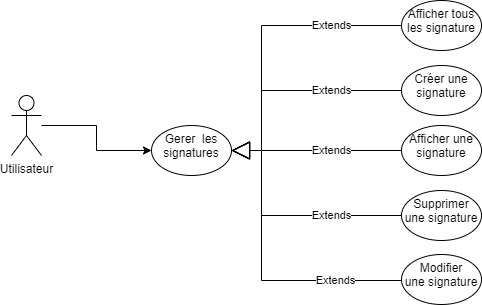
\includegraphics[width=0.8\textwidth]{use_case_signature_sprint_2}
  \caption{Diagramme de cas d'utilisation du sprint 2 : « Gestion des signatures »}
  \label{fig:UseCaseDiagram}
\end{figure}

\subsubsection{Analyse des besoins:}
\textbf{•	Description textuelle de cas d'utilisation « Créer une signature »}

\begin{longtable}{|p{5cm}|p{10cm}|}
\hline
\textbf{Cas d'utilisation}&Créer une signature\\
\hline
\textbf{Acteurs}&Utilisateur\\
\hline
\textbf{Pré Condition}&L'utilisateur doit être authentifié\\
\hline
\textbf{Post Condition}&Création d'une signature\\
\hline
\textbf{Scénario Nominal}&
\vspace{-\baselineskip}
\begin{enumerate}
    \setcounter{enumi}{1}
  \item L'utilisateur dessine sa signature sur le pad.
  \item L'utilisateur clique sur le bouton enregistrer.
  \item Le système affiche un panneau d'ajout de nom.
  \item L'utilisateur entre le nom de la signature.
  \item L'utilisateur clique sur le bouton enregistrer.
  \item Le système enregistre la signature.
  \item Le système affiche un message de succès.
  \item Le system cache le panneau d'ajout de nom.
\end{enumerate}\\
\hline
\textbf{Scénario Alternatif}&
\vspace{-\baselineskip}
\begin{enumerate}
      \item [2.1] L'utilisateur ne dessine pas sa signature sur le pad.
      \item [2.2] Le système affiche un message d'erreur pour s'assurer de dessiner la signature.
      \item [5.1] L'utilisateur ne donne pas de nom à la signature.
      \item [5.2] Le système affiche un message d'erreur pour s'assurer de donner un nom à la signature.
\end{enumerate}\\
\hline
\textbf{Scénario d'exception}&Erreur de connexion\\
\hline
\caption{Description textuelle du diagramme de cas d'utilisation « Créer une signature »}
\label{tab:use_case_create_signature}
\end{longtable}

% \textbf{Terminologie paragraphe :} \\
% \textbf{OCR :} signifie Optical Character Recognition (reconnaissance optique de caractères en français). Il s'agit d'un processus de conversion d'images numérisées de textes en fichiers éditables et interprétables par des ordinateurs.
  

\textbf{•	Description textuelle de cas d'utilisation « Afficher les signatures »}

\begin{longtable}{|p{5cm}|p{10cm}|}
\hline
\textbf{Cas d'utilisation}&Afficher les signatures\\
\hline
\textbf{Acteurs}&Utilisateur \\
\hline
\textbf{Pré Condition}&L'utilisateur doit être authentifié\\
\hline
\textbf{Post Condition}&Affichage des signatures\\
\hline
\textbf{Scénario Nominal}&
\vspace{-\baselineskip}
\begin{enumerate}
    \setcounter{enumi}{1}
    \item L'utilisateur clique sur le bouton « Signatures ».
    \item Le système affiche la liste des signatures.
\end{enumerate}\\
\hline
\textbf{Scénario alternatif}&
\begin{enumerate}
  \item [2.1] L'utilisateur n'a pas de signature.
  \item [2.2] Le système affiche un message pour l'inviter à créer une signature.
\end{enumerate}\\
\hline
\textbf{Scénario d'exception}&Erreur de connexion\\
\hline
\caption{Description textuelle du diagramme de cas d'utilisation « Afficher les signatures »}
\label{tab:use_case_view_signature}
\end{longtable}


\textbf{•	Description textuelle de cas d'utilisation « Supprimer une signature »}

\begin{longtable}{|p{5cm}|p{10cm}|}
\hline
\textbf{Cas d'utilisation}&Supprimer une signature\\
\hline
\textbf{Acteurs}&Utilisateur \\
\hline
\textbf{Pré Condition}&L'utilisateur doit être authentifié et avoir des signatures.\\
\hline
\textbf{Post Condition}&Suppression  d'une signature\\
\hline
\textbf{Scénario Nominal}&
\vspace{-\baselineskip}
\begin{enumerate}
    \setcounter{enumi}{1}
    \item L'utilisateur clique sur le bouton supprimer.
    \item Le système affiche une alerte de vérification.
    \item L'utilisateur clique sur le bouton confirme.
    \item La signature est supprimer de la base.
    \item Le système affiche un message de succès.
\end{enumerate}\\
\hline
\textbf{Scénario d'exception}&Erreur de connexion\\
\hline
\caption{Description textuelle du diagramme de cas d'utilisation « Supprimer une signature »}
\label{tab:use_case_delete_signature}
\end{longtable}


\textbf{•	Description textuelle de cas d'utilisation « Visualiser une signature »}

\begin{longtable}{|p{5cm}|p{10cm}|}
\hline
\textbf{Cas d'utilisation}&Visualiser une signature\\
\hline
\textbf{Acteurs}&Utilisateur \\
\hline
\textbf{Pré Condition}&L'utilisateur doit être authentifié et avoir des signatures.\\
\hline
\textbf{Post Condition}&Visualisation d'une signature\\
\hline
\textbf{Scénario Nominal}&
\vspace{-\baselineskip}
\begin{enumerate}
    \setcounter{enumi}{1}
    \item L'utilisateur clique sur le bouton visualiser.
    \item Le système affiche la signature.
\end{enumerate}\\
\hline
\textbf{Scénario d'exception}&Erreur de connexion\\
\hline
\caption{Description textuelle du diagramme de cas d'utilisation « Visualiser une signature »}
\label{tab:use_case_view_single_signature}
\end{longtable}


\textbf{•	Description textuelle de cas d'utilisation « Créer une signature a l'aide du caméra ou d'image »}
\begin{longtable}{|p{5cm}|p{10cm}|}
\hline
\textbf{Cas d'utilisation}&Créer une signature a l'aide du caméra ou d'image\\
\hline
\textbf{Acteurs}&Utilisateur \\
\hline
\textbf{Pré Condition}&L'utilisateur doit être authentifié.\\
\hline
\textbf{Post Condition}&Création d'une signature\\
\hline
\textbf{Scénario Nominal}&
\vspace{-\baselineskip}
\begin{enumerate}
    \setcounter{enumi}{1}
    \item L'utilisateur clique sur le bouton Importer.
    \item Le système affiche une fenêtre pour choisir ou prendre une image.
    \item L'utilisateur choisit l'image.
    \item Le système affiche l'image pour que l'utilisateur puisse la redimensionner.
    \item L'utilisateur redimensionne l'image.
    \item Le système récupère la signature de la partie de l'image choisie et l'affiche pour que l'utilisateur puisse la modifier.
    \item L'utilisateur modifie la signature.
    \item Le systeme procède à la création de la signature. // TODO !!
\end{enumerate}\\
\hline
\textbf{Scénario alternatif}&
\begin{enumerate}
  \item [2.1] L'utilisateur choisit une fichier qui n'est pas une image.
  \item [2.2] Le système affiche un message d'erreur.
  \item [4.1] L'utilisateur annule la redimension.
  \item [4.2] Le scenario reprend à l'étape 2.
\end{enumerate}\\
\hline
\textbf{Scénario d'exception}&Erreur de connexion\\
\hline
\caption{Description textuelle du diagramme de cas d'utilisation « Créer une signature a l'aide du caméra ou d'image »}
\label{tab:use_case_create_signature_from_image}
\end{longtable}

Pour créer notre plateforme, nous avons pensé qu'il était nécessaire de réaliser une maquette. Les maquettes nous aident à concevoir des interfaces qui répondent aux attentes et aux besoins du client. Elles permettent également de s'assurer que les besoins du client sont adaptés au projet. Nous avons réalisé un prototype de notre système, comme le montrent les figures ci-dessous. Tout au long de notre projet, nous présenterons des maquettes.

\begin{figure}[H]
  \centering
  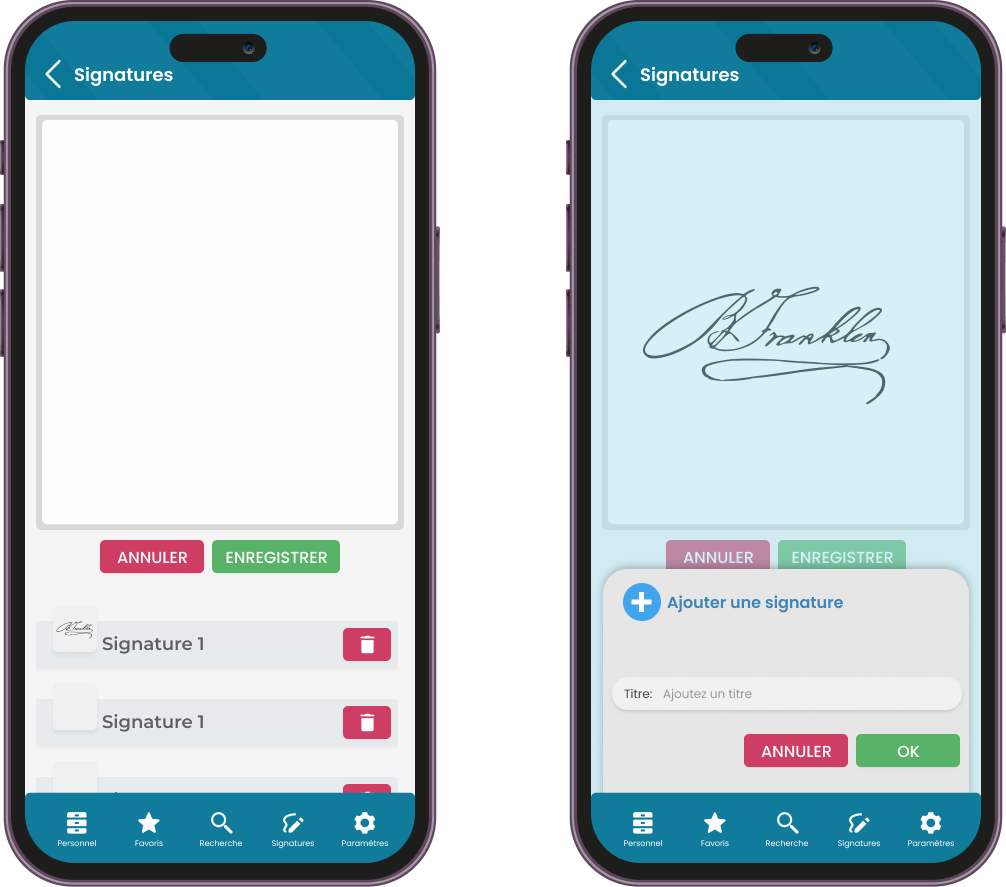
\includegraphics[width=0.7\textwidth]{design_signatures}
  \caption{Maquette de la page des signatures}
  \label{fig:design_signatures}
\end{figure}

\begin{figure}[H]
  \centering
  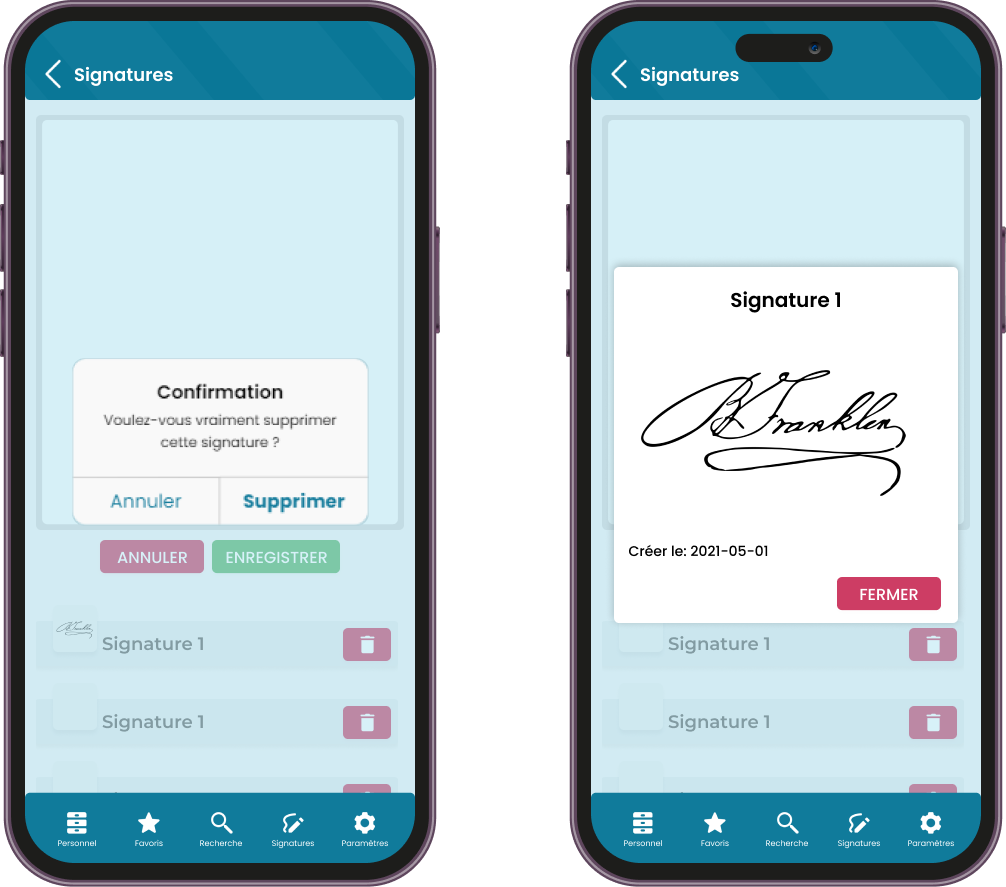
\includegraphics[width=0.7\textwidth]{preview_delete_signature}
  \caption{Maquette de la page de visualisation et de suppression d'une signature}
  \label{fig:design_preview_delete_signature}
\end{figure}

\subsubsection{Analyse détaillée}
La présentation de démarche d'analyse fonctionnelle d'un sprint est très importante pour la satisfaction d'un client parce qu'elle consiste à caractériser les fonctions offertes par un produit.
Donc, nous allons faire l'analyse des différents cas d'utilisation en utilisant le diagramme de classes d'analyse.

//TODO: ADD DIAGRAMME DE CLASSE ANALYSE
// TODO: ADD DIAGRAMMEs

\subsubsection{Conception}

Après la présentation des diagrammes d'analyse, nous avons présenté dans cette partie les diagrammes de conception.
Nous allons présenter dans cette partie les diagrammes de conception de sprint 2.

\textbf{•	Diagramme de classe de conception de sprint 2 : « Gestion des signatures »}

% add image
\begin{figure}[H]
  \centering
  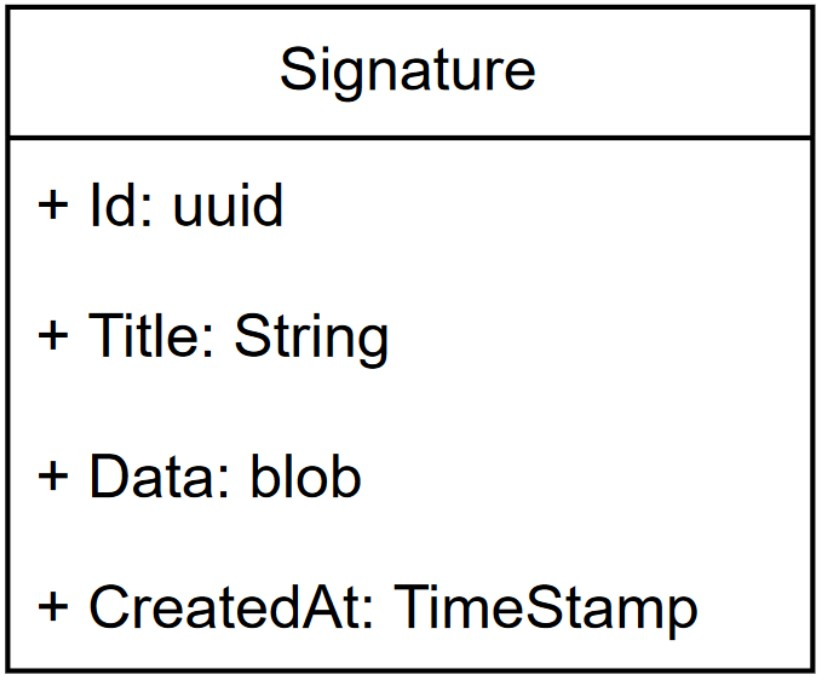
\includegraphics[width=0.35\textwidth, height=0.35\textheight]{class_diagram_signatures}
  \caption{Diagramme de classe de conception de sprint 2 : « Gestion des signatures »}
  \label{fig:class_diagram_signatures}
\end{figure}

\subsubsection{Réalisation}

Après la présentation des diagrammes d'analyse, nous avons présenté dans cette partie des captures d'écran de l'application.

\textbf{•	Interface de création d'une signature:}

Cette capture d'écran, représente l'interface de création d'une signature par un utilisateur

% add image
\begin{figure}[H]
  \centering
  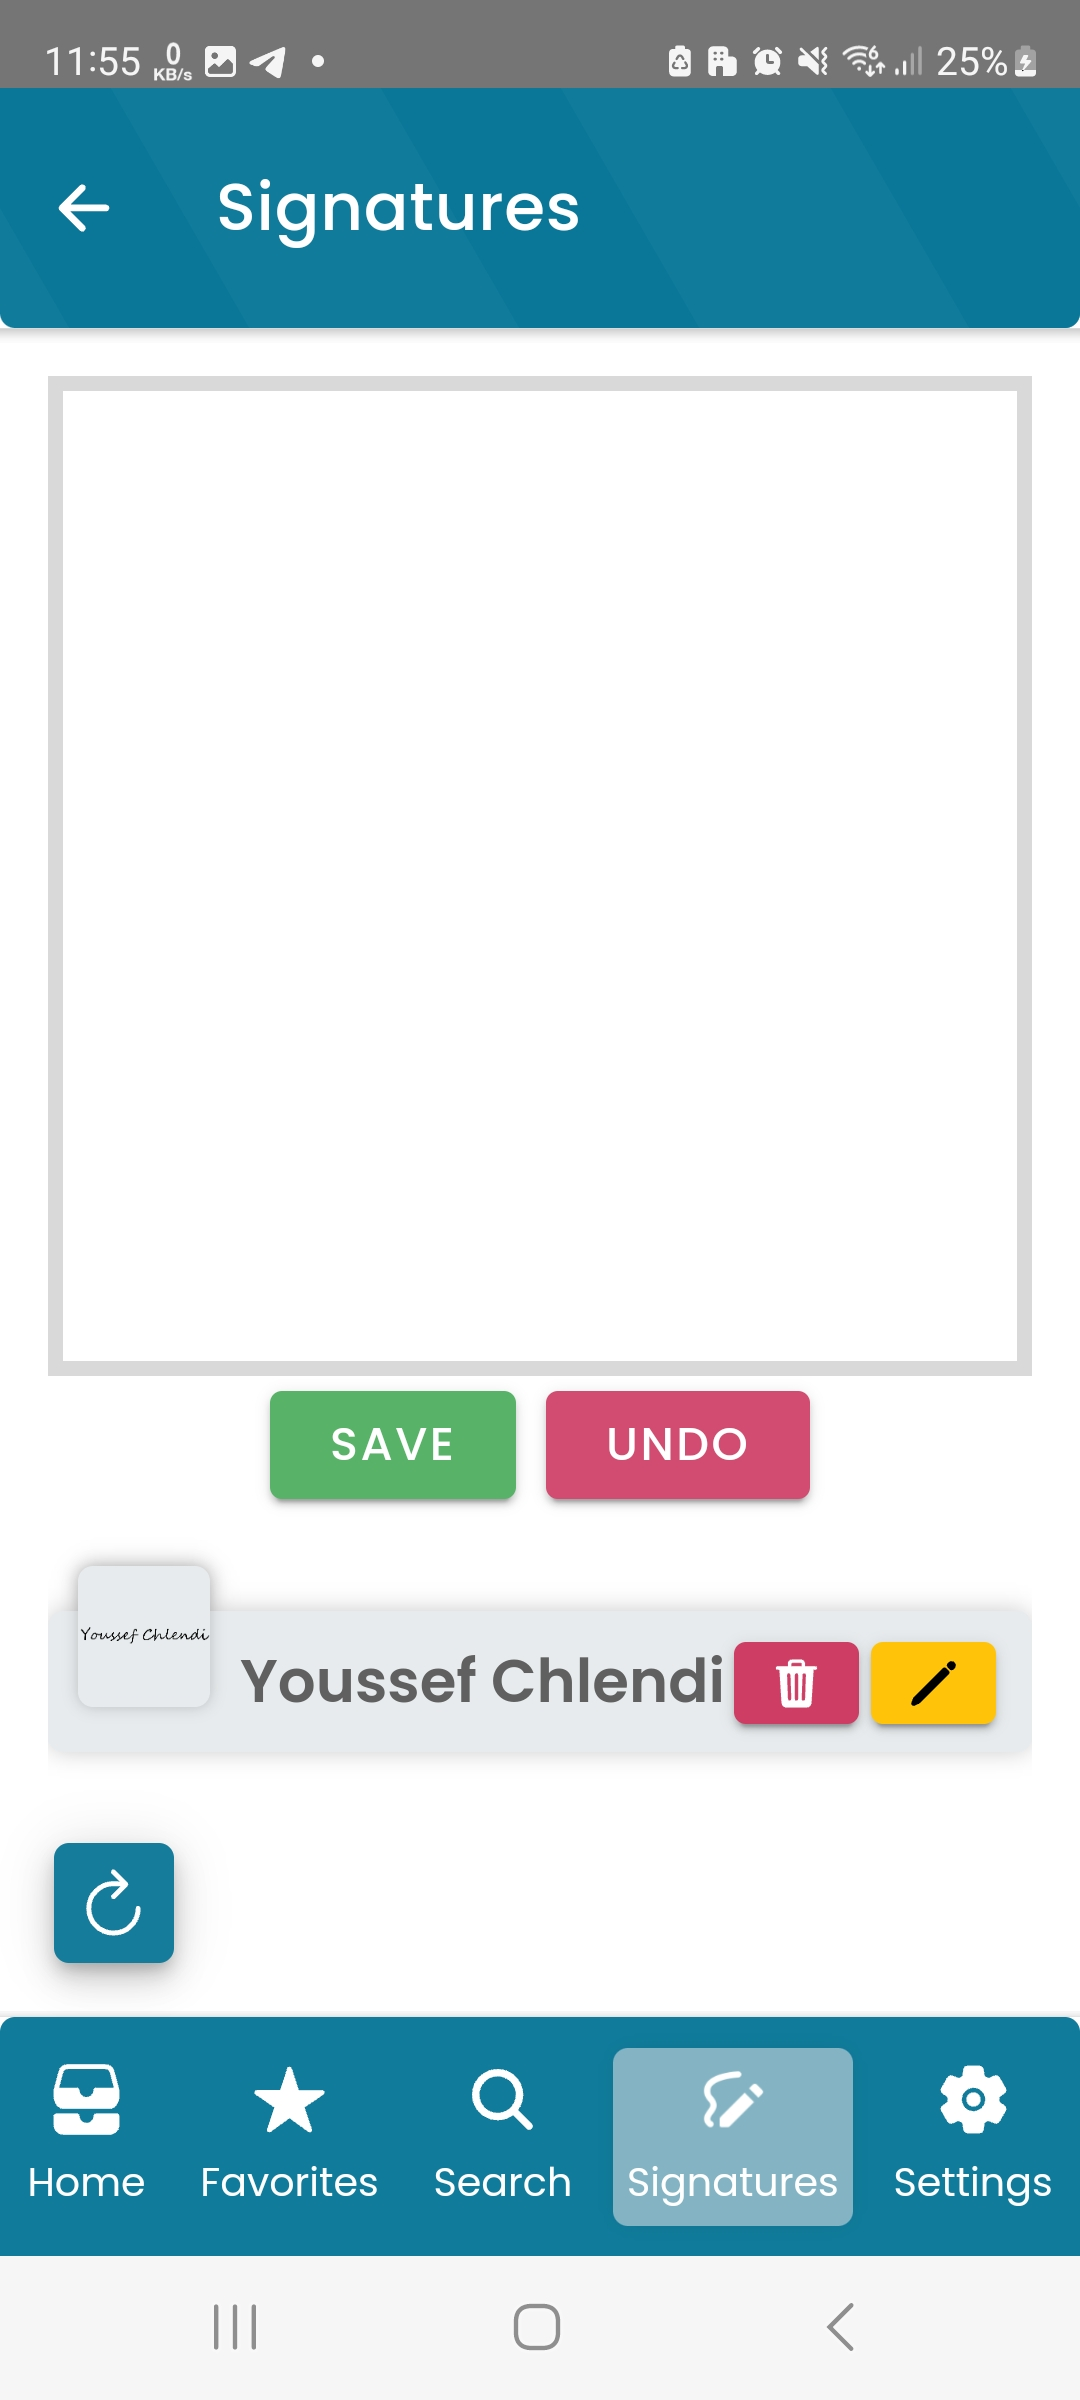
\includegraphics[width=0.35\textwidth, height=0.35\textheight,keepaspectratio=true]{signature_creation}
  \caption{Interface de création d'une signature}
  \label{fig:signature_creation}
\end{figure}

\textbf{•	Signer puis cliquer sur « save » : Interface de saisie du titre:}\\
Cette capture d'écran, représente l'interface de saisie du titre de la signature par un utilisateur
% add image
\begin{figure}[H]
  \centering
  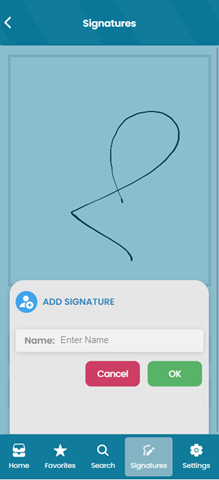
\includegraphics[width=0.35\textwidth, height=0.35\textheight,keepaspectratio=true]{signature_form}
  \caption{Interface de saisie du titre de la signature}
  \label{fig:signature_title}
\end{figure}

\textbf{•	Interface de visualisation d'une signature:}\\
Cette capture d'écran, représente l'interface de visualisation d'une signature par un utilisateur

% add image
\begin{figure}[H]
  \centering
  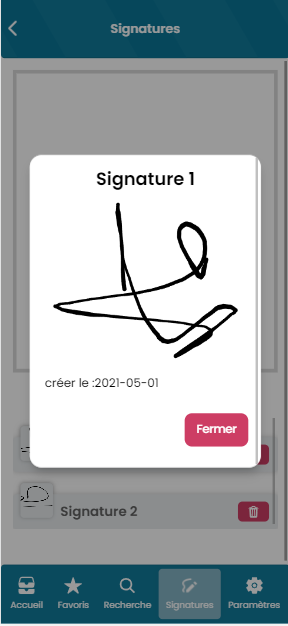
\includegraphics[width=0.35\textwidth, height=0.35\textheight,keepaspectratio=true]{signature_preview}
  \caption{Interface de visualisation d'une signature}
  \label{fig:signature_view}
\end{figure}

\textbf{•	Interface de suppression d'une signature:}\\
Cette capture d'écran, représente l'interface de suppression d'une signature par un utilisateur

% add image
\begin{figure}[h!]
  \centering
  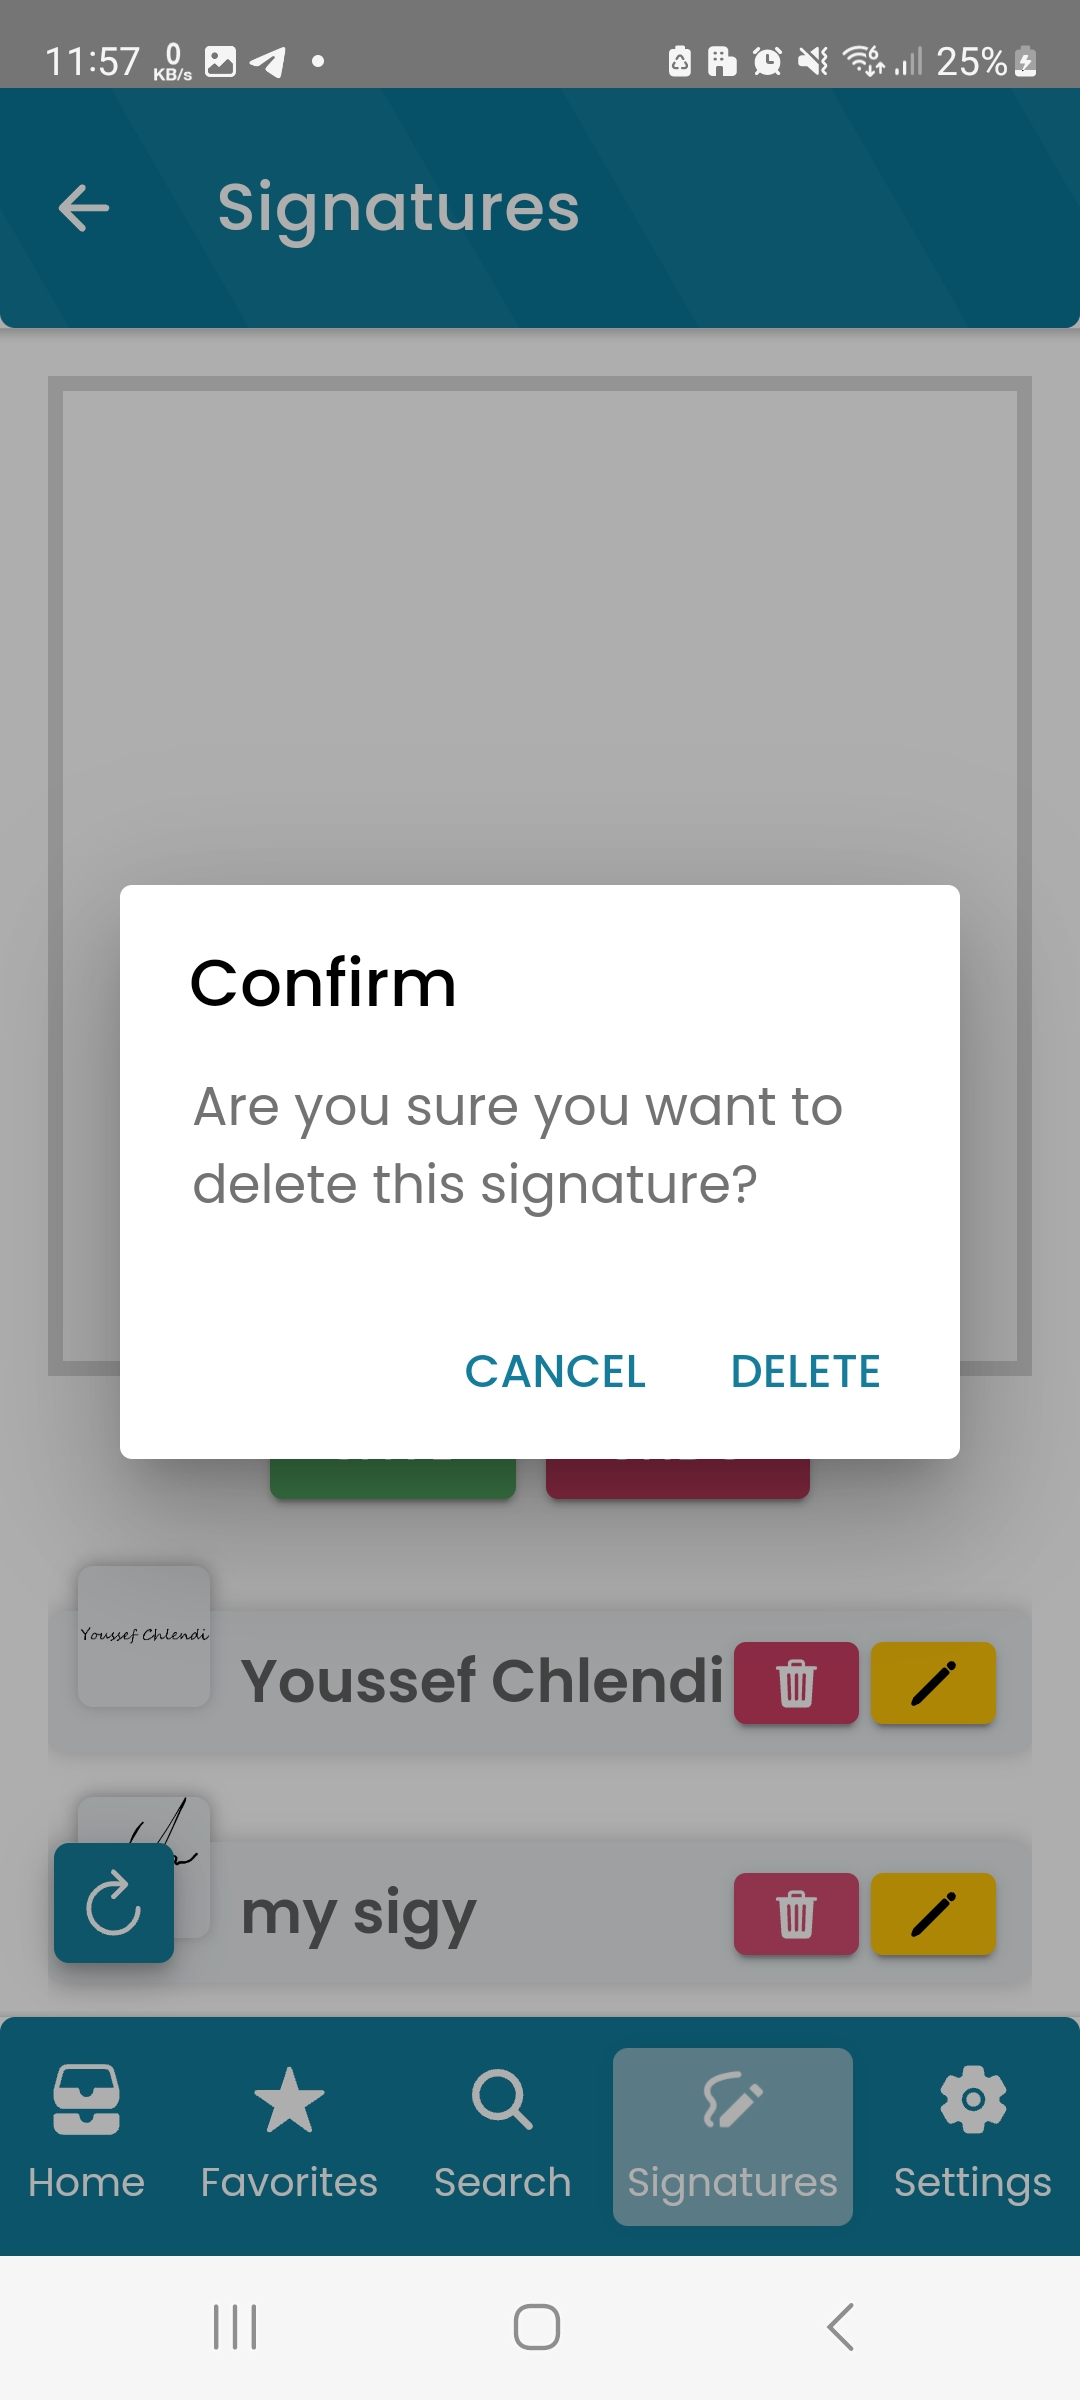
\includegraphics[width=0.35\textwidth, height=0.35\textheight,keepaspectratio=true]{signature_delete}
  \caption{Interface de suppression d'une signature}
  \label{fig:signature_delete}
\end{figure}



\subsection{Sprint Review:}
A la fin de ce sprint, nous avons planifié une réunion dans la société Neoledge afin de vérifier notre démarche de travail par rapport au besoin de client tout en respectant le délai que nous avons prévu.

Nous avons fait une démonstration durant laquelle nous allons présenter notre incrément :

\begin{itemize}
  \item La création d'une signature.
  \item La visualisation de la signature.
  \item La suppression de la signature.
\end{itemize}

\subsection{Sprint retrospective:}

Après la Sprint Review, nous avons réfléchi à des pistes pour améliorer la qualité et l'efficacité de notre application.

\noindent\textbf{•	Ce qui s'est bien passé :}
\begin{itemize}
  \item Nous avons bien partagé les tâches entre nous à travers le logiciel Azure DevOps. 
  \item Nous avons terminé le sprint dans le délai.
\end{itemize}

\noindent\textbf{•	Ce qui s'est mal passé :}
\begin{itemize}
  \item L'intégration du bibliothèque vue-signature-pad
  \item Un problème rencontré lors de la sauvegarde de la signature était que l'image enregistrée occupait la totalité de l'espace du pad, ce qui nécessitait ensuite une étape de découpe pour obtenir uniquement la partie signée.
\end{itemize}

% sprint =3
\section{Sprint 3 « Gestion des documents »}
\subsection{Sprint Goal:}

L'objectif de ce sprint est de développer et mettre en place un système de gestion des documents permettant aux utilisateurs de consulter les informations du document, consulter et gérer un fichier dans un document, consulter et gérer les tâches dans un document, chercher un document et consulter la liste des documents en favoris

\pagebreak

\subsection{Sprint Backlog « Gestion des documents »}

\begin{longtable}{|p{4cm}|p{7cm}|p{2cm}|p{2cm}|}
  \hline
  \textbf{Les items} &\textbf{Les tâches} & \textbf{Période} & \textbf{Sprint} \\
  \hline
  \vspace{-\baselineskip}
  \begin{enumerate}
    \setcounter{enumi}{1}
    \itemsep0em 
      \item Accéder à un document.
      \item Consulter la liste des fichiers d'un document
      \item Ajoutez un fichier à un document.
      \item Supprimer un fichier d'un document.
      \item Consulter la liste des tâches d'un document.
      \item Démarrer une tâche.
      \item Terminer une tâche.
      \item Consulter la liste des documents en favoris.
      \item Chercher un document.
      

  \end{enumerate}
  &
  \vspace{-\baselineskip}
  \begin{itemize}
    \itemsep0em 
    \item Préparer les interfaces sur Figma.
    \item Développer l'interface des favoris.
    \item Développer l'interface des documents.
    \item Développer l'interface de recherche de documents.
    \item Développer l'interface de liste des fichiers.
    \item Développer l'interface de liste des tâches.
    \item Développer une fonction qui permet de récupérer la liste des documents d'une base de donner.
    \item Développer une fonction qui permet de récupérer la liste des documents en favoris.
    \item Développer une fonction qui permet de chercher un document.
    \item Développer une fonction qui permet ajouter un fichier à un document.
    \item Développer une fonction qui permet de supprimer un fichier.
    \item Développer une fonction qui permet de démarrer une tâche d'un document.
    \item Développé une fonction qui permet de terminer une tâche.

  \end{itemize}
  &
  De 8 à 15 février  
  &
  3
  \\
  \hline
  \caption{Product Backlog Sprint 3}
  \label{tab:product_backlog_sprint_3}



\end{longtable}


\subsection{Implémentation du Sprint 3}
\textbf{•	Diagramme de cas d'utilisation du sprint 3 : « Gestion des documents »}

% add image
\begin{figure}[H]
  \centering
  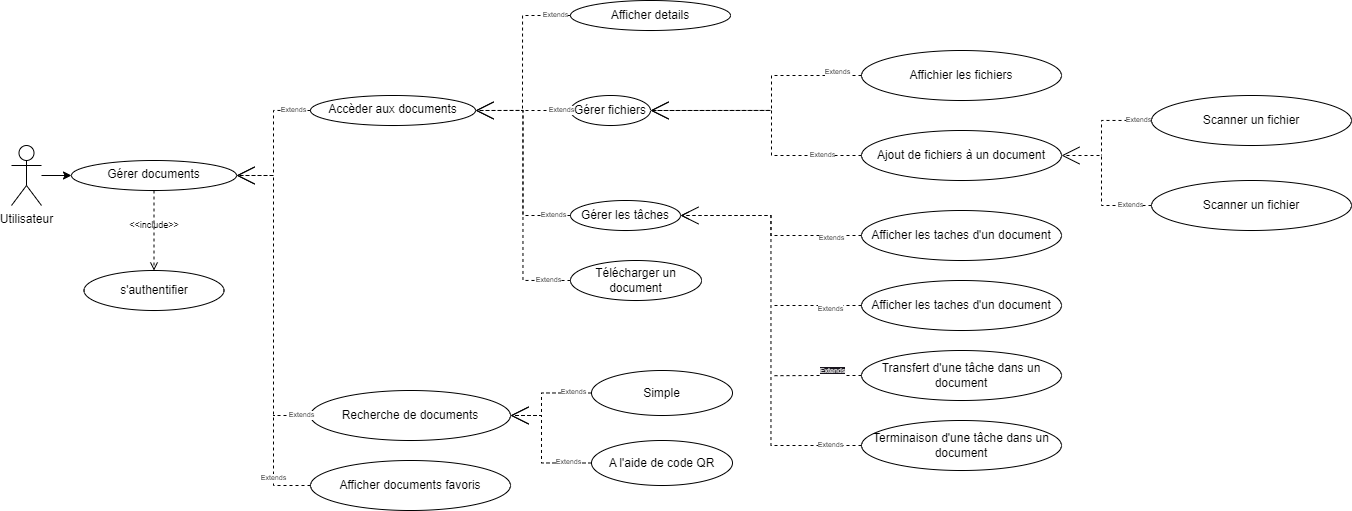
\includegraphics[width=0.8\textwidth]{use_case_documents_sprint_3}
  \caption{Diagramme de cas d'utilisation du sprint 3 : « Gestion des documents »}
  \label{fig:UseCaseDiagramSprint3}
\end{figure}


\subsubsection{Analyse des besoins:}
\textbf{•	Description textuelle de cas d'utilisation « Accéder à un document »}

\begin{longtable}{|p{5cm}|p{10cm}|}
\hline
\textbf{Cas d'utilisation}&Accéder à un document\\
\hline
\textbf{Acteurs}&Utilisateur\\
\hline
\textbf{Pré Condition}&Le document existe\\
\hline
\textbf{Post Condition}&Consultation d'un document\\
\hline
\textbf{Scénario Nominal}&
\vspace{-\baselineskip}
\begin{enumerate}
    \setcounter{enumi}{1}
    \item L'utilisateur clique sur le document.
    \item Le système affiche l'interface de document.
    
\end{enumerate}\\
\hline
\textbf{Scénario Alternatif}&
\vspace{-\baselineskip}
\begin{enumerate}
    \setcounter{enumi}{2}
    \item Aucun résultat.
\end{enumerate}\\
\hline
\textbf{Scénario d'exception}&Erreur de connexion\\
\hline
\end{longtable}


\textbf{•	Description textuelle de cas d'utilisation « consulter la liste des fichiers d'un document »}

\begin{longtable}{|p{5cm}|p{10cm}|}
\hline
\textbf{Cas d'utilisation}&Consulter la liste des fichiers d'un document\\
\hline
\textbf{Acteurs}&Utilisateur\\
\hline
\textbf{Pré Condition}&Le document existe\\
\hline
\textbf{Post Condition}&Consultation de la liste des fichiers\\
\hline
\textbf{Scénario Nominal}&
\vspace{-\baselineskip}
\begin{enumerate}
    \setcounter{enumi}{1}
    \item L'utilisateur clique sur le bouton fichier.
    \item Le système affiche l'interface de la liste des fichiers.
    
\end{enumerate}\\
\hline
\textbf{Scénario Alternatif}&
\vspace{-\baselineskip}
\begin{enumerate}
    \setcounter{enumi}{2}
    \item Aucun résultat.
\end{enumerate}\\
\hline
\textbf{Scénario d'exception}&Erreur de connexion\\
\hline
\end{longtable}

\textbf{•	Description textuelle de cas d'utilisation « ajouter un fichier à un document »}

\begin{longtable}{|p{5cm}|p{10cm}|}
\hline
\textbf{Cas d'utilisation}&Ajouter un fichier à un document\\
\hline
\textbf{Acteurs}&Utilisateur\\
\hline
\textbf{Pré Condition}&Le document existe\\
\hline
\textbf{Post Condition}&Fichier ajouté\\
\hline
\textbf{Scénario Nominal}&
\vspace{-\baselineskip}
\begin{enumerate}
    \setcounter{enumi}{1}
    \item L'utilisateur clique sur le bouton ajouter.
    \item Le système affiche l'interface d'ajout des fichiers.
    \item L'utilisateur ajoute le fichier et clique sur le bouton confirmer.
    \item le système affiche un message des succès.
    
    
\end{enumerate}\\
\hline
\textbf{Scénario Alternatif}&
\vspace{-\baselineskip}
\begin{enumerate}
    \setcounter{enumi}{3}
    \item L'utilisateur annule l'ajout du fichier.
\end{enumerate}\\
\hline
\textbf{Scénario d'exception}&Erreur de connexion\\
\hline
\end{longtable}


\textbf{•	Description textuelle de cas d'utilisation « supprimer un fichier dans un document »}

\begin{longtable}{|p{5cm}|p{10cm}|}
\hline
\textbf{Cas d'utilisation}&Supprimer un fichier d'un document\\
\hline
\textbf{Acteurs}&Utilisateur\\
\hline
\textbf{Pré Condition}&Le document existe\\
\hline
\textbf{Post Condition}&Fichier supprimé\\
\hline
\textbf{Scénario Nominal}&
\vspace{-\baselineskip}
\begin{enumerate}
    \setcounter{enumi}{1}
    \item L'utilisateur clique sur le bouton supprimer.
    \item Le système affiche une alerte de confirmation.
    \item L'utilisateur clique sur le bouton confirmer.
    \item le système supprime le fichier et affiche un message des succès.
    
    
    
\end{enumerate}\\
\hline
\textbf{Scénario Alternatif}&
\vspace{-\baselineskip}
\begin{enumerate}
    \setcounter{enumi}{3}
    \item L'utilisateur annule la suppression du fichier.
\end{enumerate}\\
\hline
\textbf{Scénario d'exception}&Erreur de connexion\\
\hline
\end{longtable}



\textbf{•	Description textuelle de cas d'utilisation « consulter la liste des tâches d'un document »}

\begin{longtable}{|p{5cm}|p{10cm}|}
\hline
\textbf{Cas d'utilisation}&Consulter la liste des tâches d'un document\\
\hline
\textbf{Acteurs}&Utilisateur\\
\hline
\textbf{Pré Condition}&Le document existe\\
\hline
\textbf{Post Condition}&Consultation des tâches\\
\hline
\textbf{Scénario Nominal}&
\vspace{-\baselineskip}
\begin{enumerate}
    \setcounter{enumi}{1}
    \item L'utilisateur clique sur le bouton tâches.
    \item Le système affiche l'interface de la liste des tâches.
    
\end{enumerate}\\
\hline
\textbf{Scénario Alternatif}&
\vspace{-\baselineskip}
\begin{enumerate}
    \setcounter{enumi}{3}
    \item Aucun tâche trouvée.
\end{enumerate}\\
\hline
\textbf{Scénario d'exception}&Erreur de connexion\\
\hline
\end{longtable}



\textbf{•	Description textuelle de cas d'utilisation « Demander une tâche »}

\begin{longtable}{|p{5cm}|p{10cm}|}
\hline
\textbf{Cas d'utilisation}&Demander une tâche\\
\hline
\textbf{Acteurs}&Utilisateur\\
\hline
\textbf{Pré Condition}&La document a au moins une tâche\\
\hline
\textbf{Post Condition}&Tâche demandée\\
\hline
\textbf{Scénario Nominal}&
\vspace{-\baselineskip}
\begin{enumerate}
    \setcounter{enumi}{1}
    \item L'utilisateur clique sur le bouton demander.
    \item Le système affiche un modal de demande de tâche.
    \item L'utilistauer rempli le formulaire.
    \item L'utilisateur clique sur le bouton confirmer.
    \item Le système cache le modal de demande de tâche.
    \item Le système affiche un message de succès.
\end{enumerate}\\
\hline
\textbf{Scénario Alternatif}&
\vspace{-\baselineskip}
\begin{enumerate}
    \setcounter{enumi}{4}
    \item L'utilisateur annule la demande de tâche.
    \item Le système cache le modal de demande de tâche.
\end{enumerate}\\
\hline
\textbf{Scénario d'exception}&Erreur de connexion\\
\hline
\end{longtable}


\textbf{•	Description textuelle de cas d'utilisation « Tranférer une tâche »}

\begin{longtable}{|p{5cm}|p{10cm}|}
\hline
\textbf{Cas d'utilisation}&Tranférer une tâche\\
\hline
\textbf{Acteurs}&Utilisateur\\
\hline
\textbf{Pré Condition}&La document a au moins une tâche\\
\hline
\textbf{Post Condition}&Tâche transférée\\
\hline
\textbf{Scénario Nominal}&
\vspace{-\baselineskip}
\begin{enumerate}
    \setcounter{enumi}{1}
    \item L'utilisateur clique sur le bouton transférer.
    \item Le système affiche un modal de transfert de tâche.
    \item L'utilistauer rempli le formulaire.
    \item L'utilisateur clique sur le bouton confirmer.
    \item Le système cache le modal de transfert de tâche.
    \item Le système affiche un message de succès.
\end{enumerate}\\
\hline
\textbf{Scénario Alternatif}&
\vspace{-\baselineskip}
\begin{enumerate}
    \setcounter{enumi}{4}
    \item L'utilisateur annule la transfert de tâche.
    \item Le système cache le modal de transfert de tâche.
\end{enumerate}\\
\hline
\textbf{Scénario d'exception}&Erreur de connexion\\
\hline
\end{longtable}

\textbf{•	Description textuelle de cas d'utilisation « Terminer une tâche »}

\begin{longtable}{|p{5cm}|p{10cm}|}
\hline
\textbf{Cas d'utilisation}&Terminer une tâche\\
\hline
\textbf{Acteurs}&Utilisateur\\
\hline
\textbf{Pré Condition}&La document a au moins une tâche\\
\hline
\textbf{Post Condition}&Tâche terminée\\
\hline
\textbf{Scénario Nominal}&
\vspace{-\baselineskip}
\begin{enumerate}
    \setcounter{enumi}{1}
    \item L'utilisateur clique sur le bouton terminer.
    \item Le système affiche un modal de confirmation de terminaison de tâche.
    \item L'utilisateur clique sur le bouton confirmer.
    \item Le système cache le modal de confirmation de terminaison de tâche.
    \item Le système affiche un message de succès.
\end{enumerate}\\
\hline
\textbf{Scénario Alternatif}&
\vspace{-\baselineskip}
\begin{enumerate}
    \setcounter{enumi}{4}
    \item L'utilisateur annule la terminaison de tâche.
    \item Le système cache le modal de confirmation de terminaison de tâche.
\end{enumerate}\\
\hline
\textbf{Scénario d'exception}&Erreur de connexion\\
\hline
\end{longtable}



\textbf{•	Description textuelle de cas d'utilisation « Consulter la liste des documents en favoris  »}

\begin{longtable}{|p{5cm}|p{10cm}|}
\hline
\textbf{Cas d'utilisation}&Consulter la liste des documents en favoris\\
\hline
\textbf{Acteurs}&Utilisateur\\
\hline
\textbf{Pré Condition}&L'utilisateur a au moins un document en favoris\\
\hline
\textbf{Post Condition}&Affichage de la liste des documents en favoris\\
\hline
\textbf{Scénario Nominal}&
\vspace{-\baselineskip}
\begin{enumerate}
    \setcounter{enumi}{1}
    \item L'utilisateur clique sur le bouton favoris.
    \item Le système affiche la liste des documents en favoris.
\end{enumerate}\\
\hline
\textbf{Scénario Alternatif}&
\vspace{-\baselineskip}
\begin{enumerate}
    \setcounter{enumi}{2}
    \item Aucun document en favoris.
\end{enumerate}\\
\hline
\textbf{Scénario d'exception}&Erreur de connexion\\
\hline
\end{longtable}




\textbf{•	Description textuelle de cas d'utilisation « Chercher un document »}

\begin{longtable}{|p{5cm}|p{10cm}|}
\hline
\textbf{Cas d'utilisation}&Chercher un document\\
\hline
\textbf{Acteurs}&Utilisateur\\
\hline
\textbf{Pré Condition}&\\
\hline
\textbf{Post Condition}&Liste des documents correspondant à la recherche\\
\hline
\textbf{Scénario Nominal}&
\vspace{-\baselineskip}
\begin{enumerate}
    \setcounter{enumi}{1}
    \item L'utilisateur clique sur le bouton rechercher.
    \item Le système affiche l'inteface de recherche des documents.
    \item L'utilisateur rempli le formulaire de recherche.
    \item Le système affiche la liste des documents correspondant à la recherche.
\end{enumerate}\\
\hline
\textbf{Scénario Alternatif}&
\vspace{-\baselineskip}
\begin{enumerate}
    \setcounter{enumi}{4}
    \item Aucun document correspondant à la recherche.
\end{enumerate}\\
\hline
\textbf{Scénario d'exception}&Erreur de connexion\\
\hline
\end{longtable}


% Analyse detaillée 
\subsubsection{Analyse détaillée}
TODO: Add diagrams d'analyse

\subsubsection{Conception}

Après la présentation des diagrammes d'analyse, nous avons présenté dans cette partie les diagrammes de conception.
Nous allons présenter dans cette partie les diagrammes de conception de sprint 3.

\textbf{•	Diagramme de classe de conception de sprint 3 : « Gestion des documents »}

% add image
\begin{figure}[H]
  \centering
  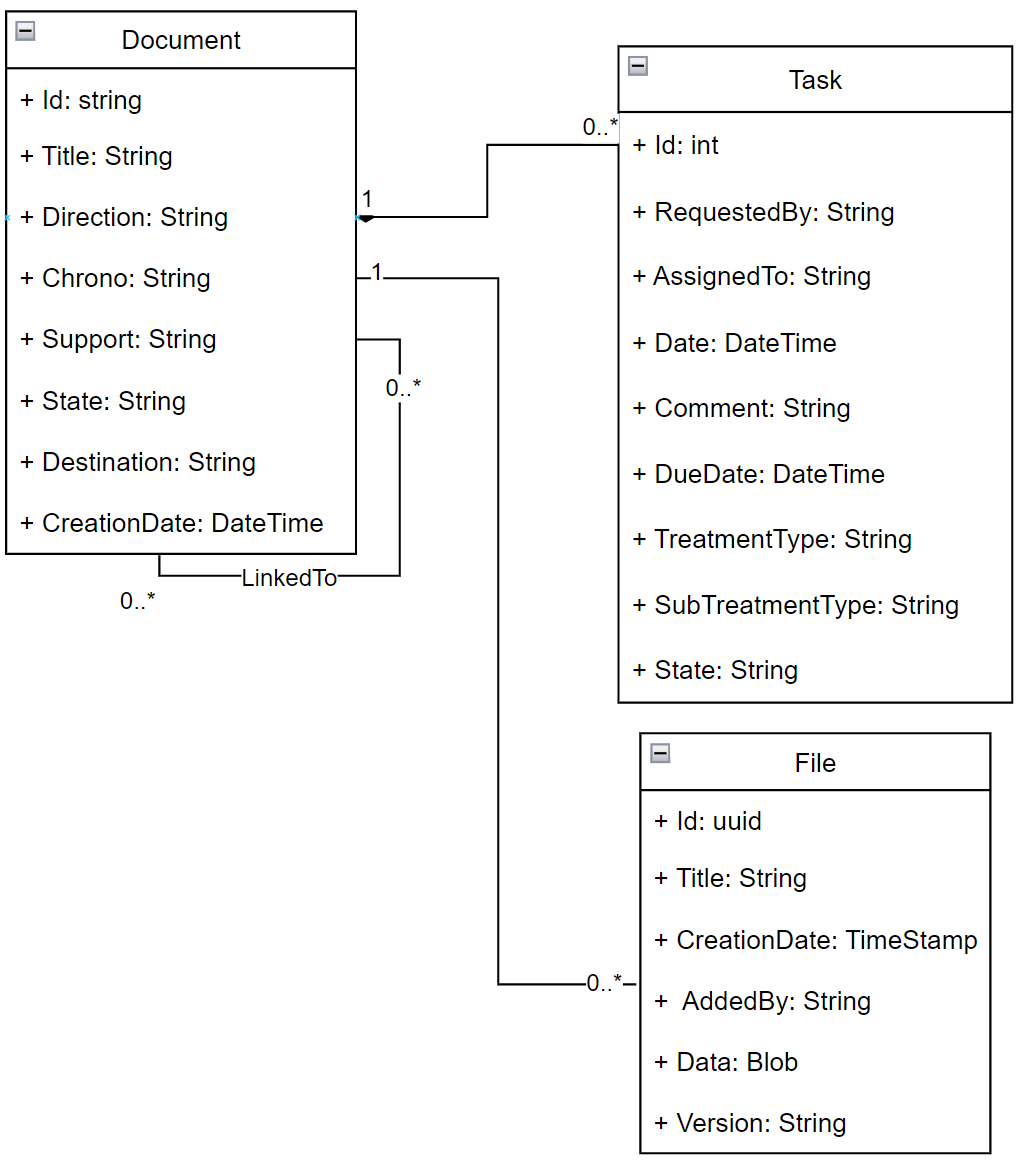
\includegraphics[width=0.8\textwidth]{class_diagram_documents.png}
  \caption{Diagramme de classe de conception de sprint 3 : « Gestion des documents »}
  \label{fig:diagramme_de_classe_de_conception_de_sprint_3_gestion_des_documents}
\end{figure}


\subsubsection{Réalisation}

Après la présentation des diagrammes d'analyse, nous avons présenté dans cette partie des captures d'écran de l'application.

\textbf{•	Accès aux documents:}

Cette capture d'écran, représente l'interface d'accès aux documents par un utilisateur

% add image
\begin{figure}[H]
  \centering
  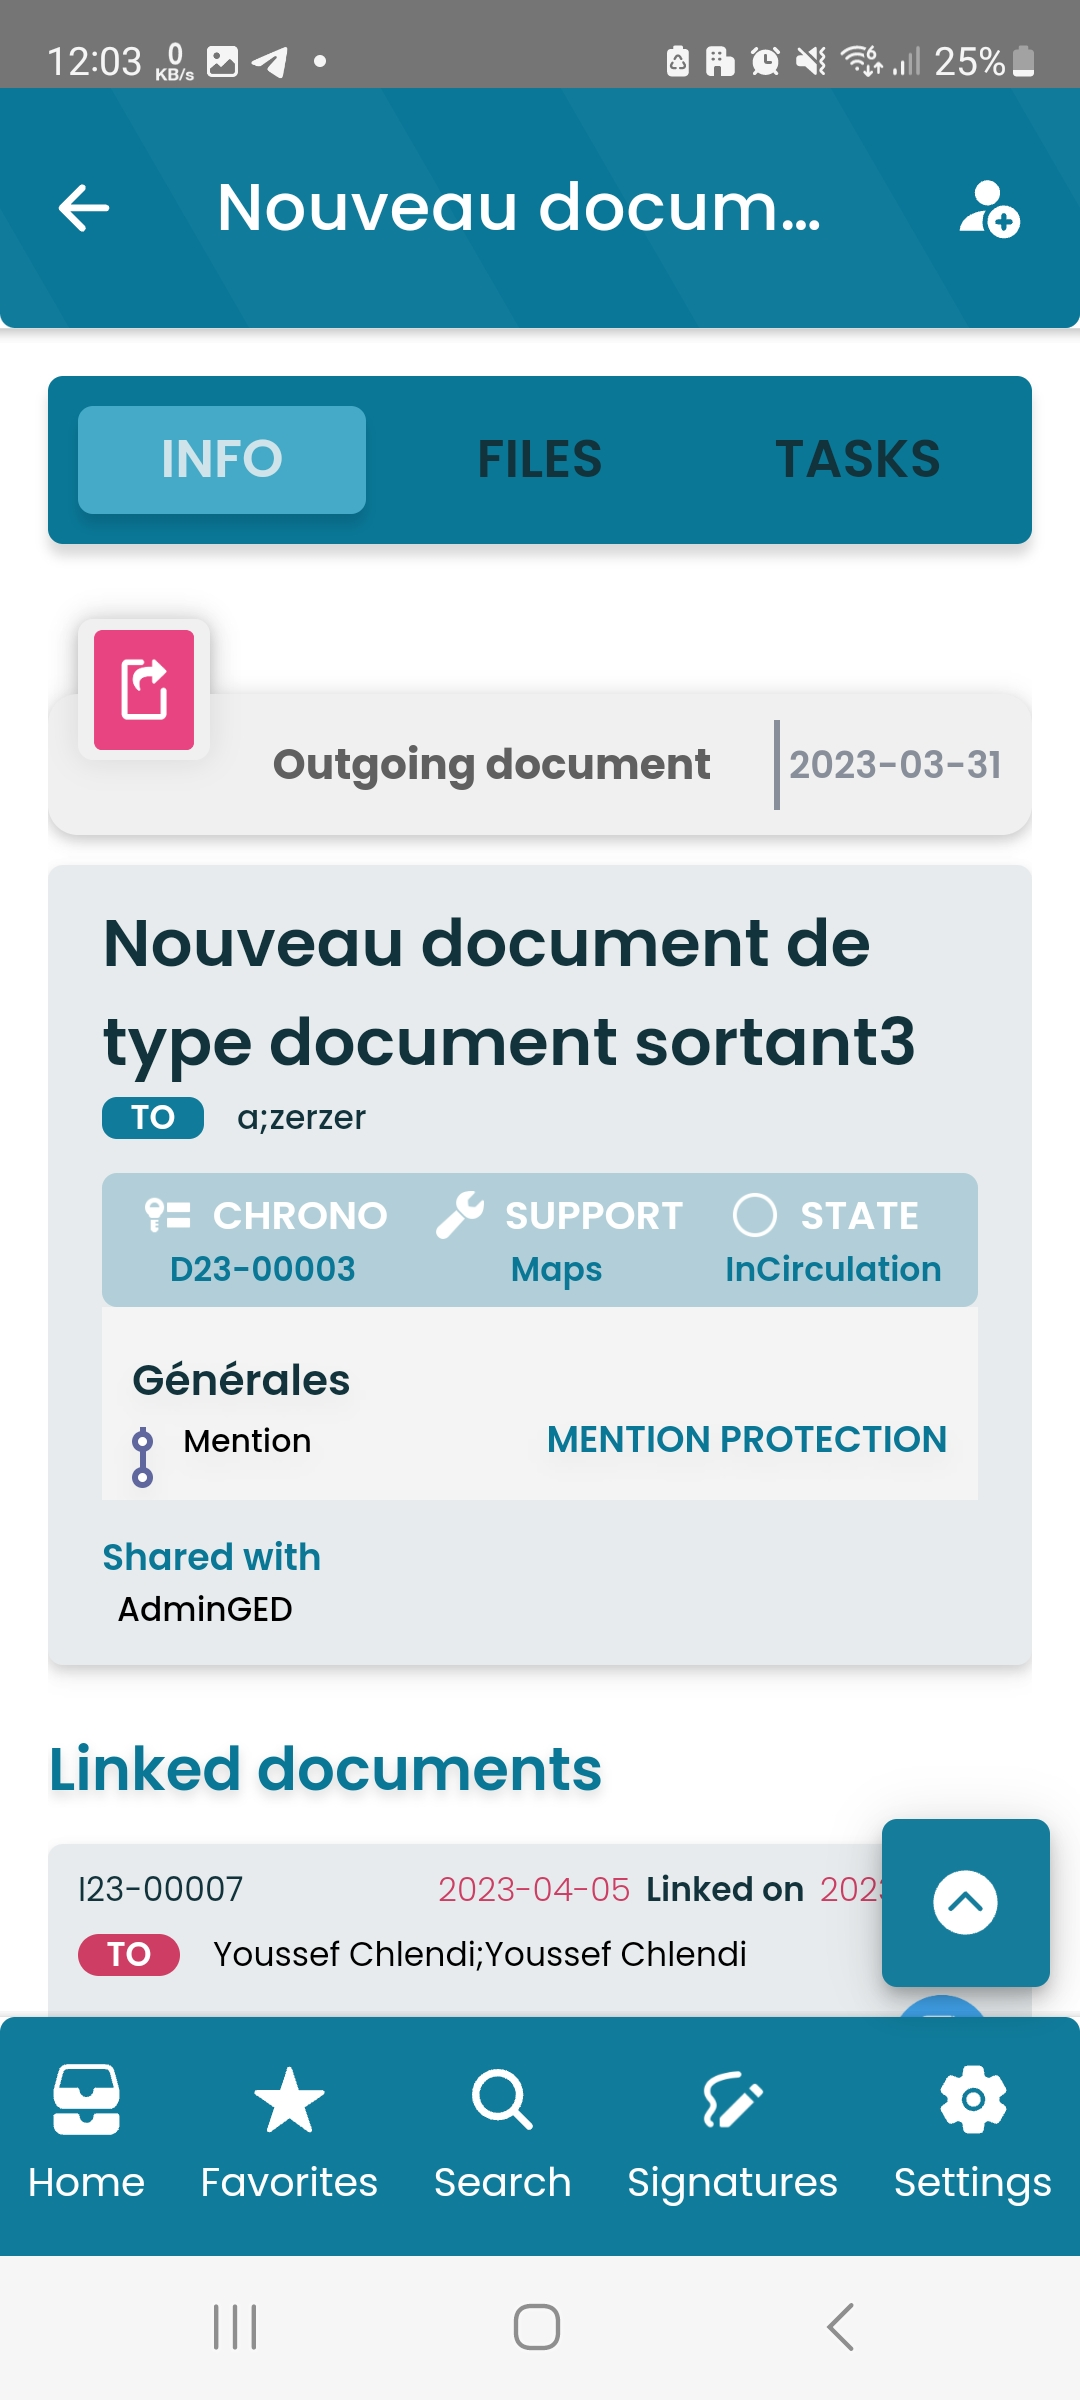
\includegraphics[width=0.35\textwidth, height=0.35\textheight,keepaspectratio=true]{acces_aux_document}
  \caption{Interface d'accès aux documents}
  \label{fig:acces_aux_document}
\end{figure}

\textbf{•	Consulter les fichiers d'un document:}

Cette capture d'écran, représente l'interface de consultation des fichiers d'un document par un utilisateur

% add image
\begin{figure}[H]
  \centering
  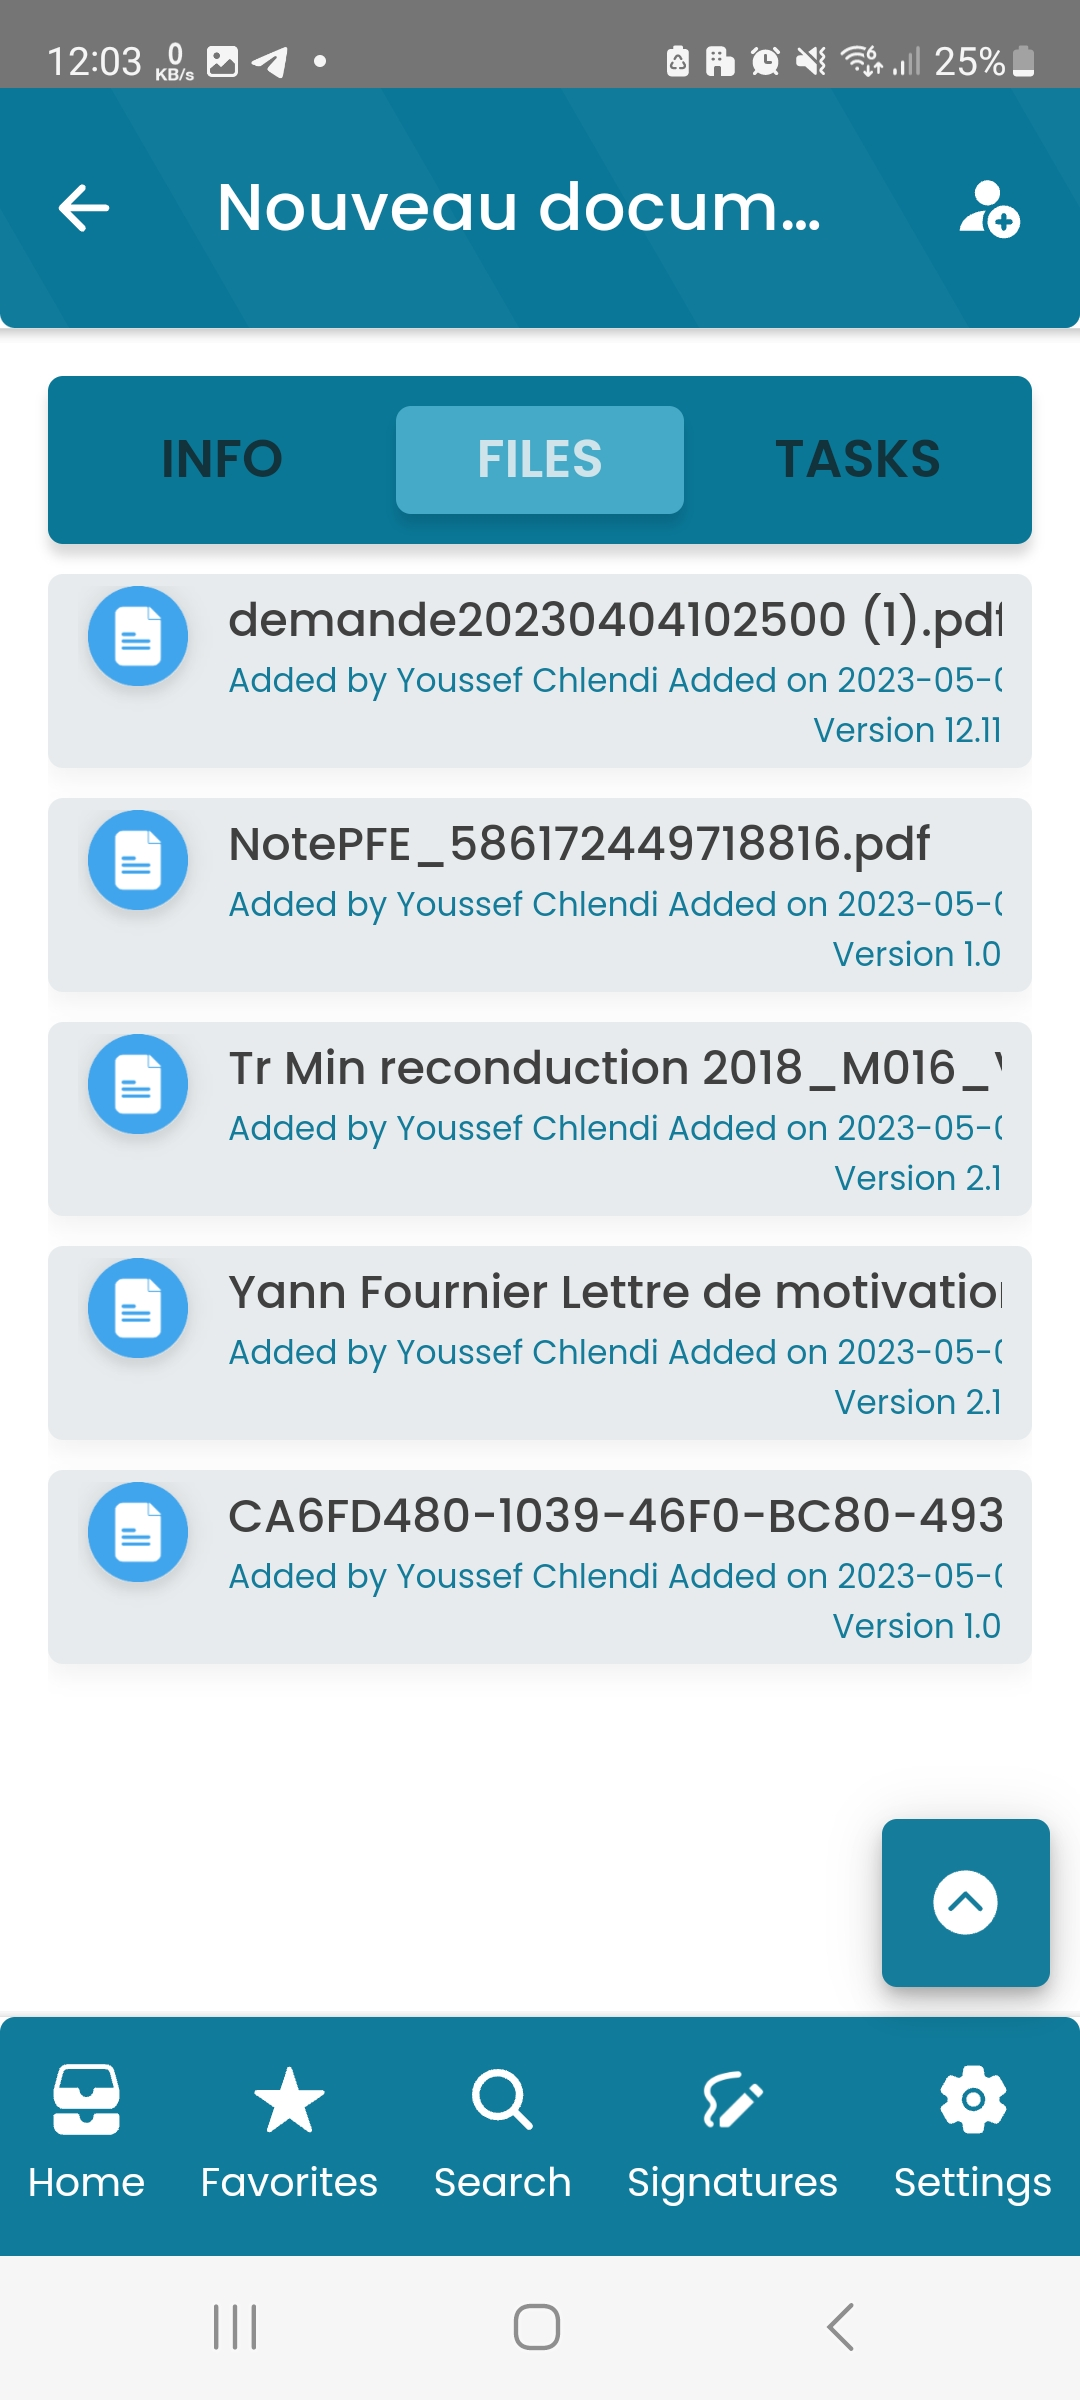
\includegraphics[width=0.35\textwidth, height=0.35\textheight,keepaspectratio=true]{consult_document_files}
  \caption{Interface de consultation des fichiers d'un document}
  \label{fig:consult_document_files}
\end{figure}

\textbf{•	Consulter les tâches d'un document:}

Cette capture d'écran, représente l'interface de consultation des tâches d'un document par un utilisateur

% add image
\begin{figure}[H]
  \centering
  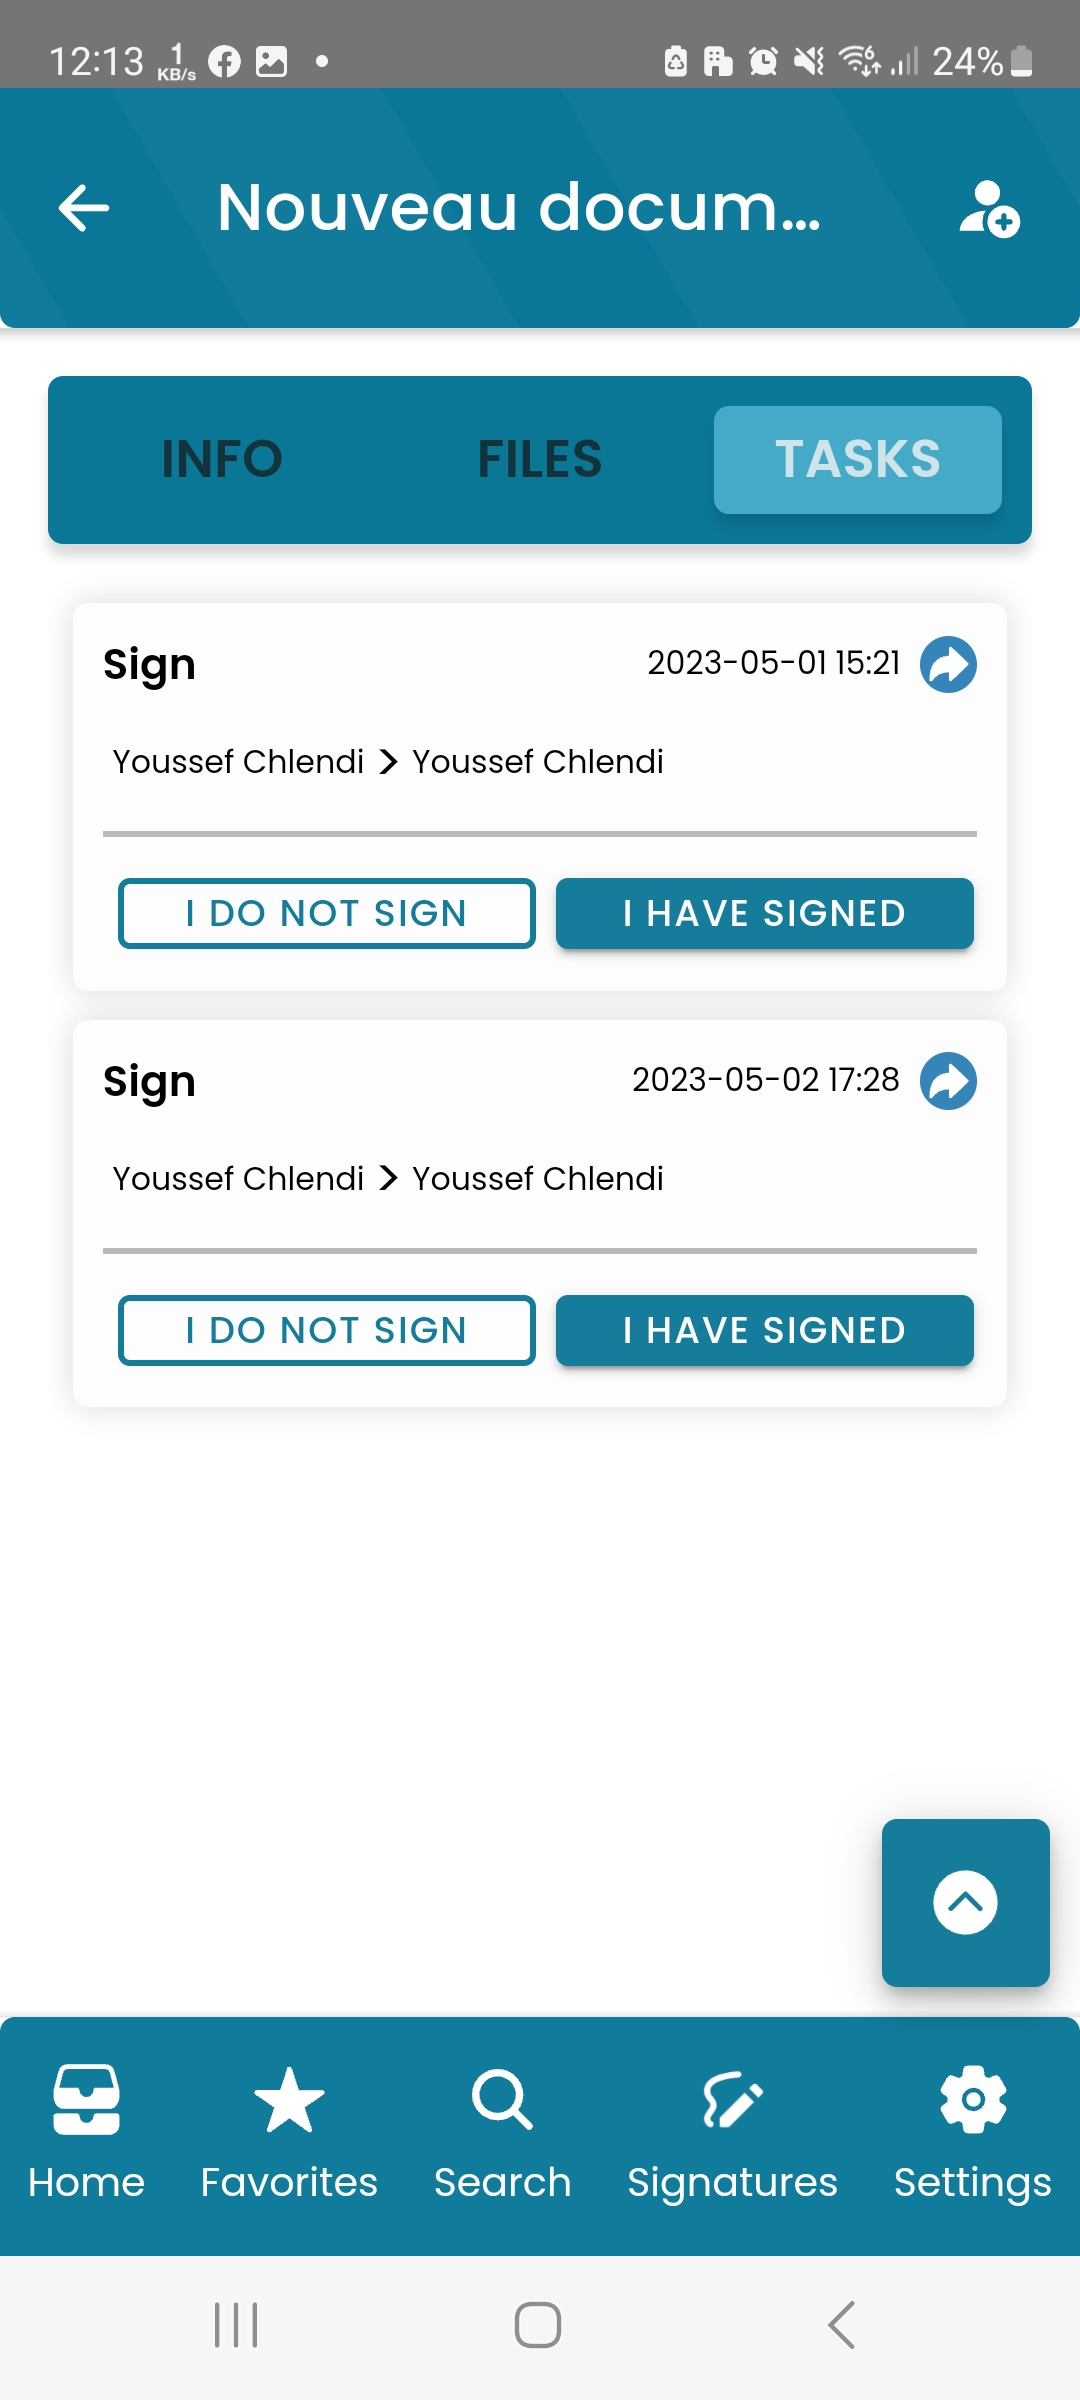
\includegraphics[width=0.35\textwidth, height=0.35\textheight,keepaspectratio=true]{consult_document_tasks}
  \caption{Interface de consultation des tâches d'un document}
  \label{fig:consult_document_tasks}
\end{figure}

\textbf{•	Ajout de fichiers à un document:}

Cette capture d'écran, représente l'interface d'ajout de fichiers à un document par un utilisateur

% add image
\begin{figure}[H]
  \centering
  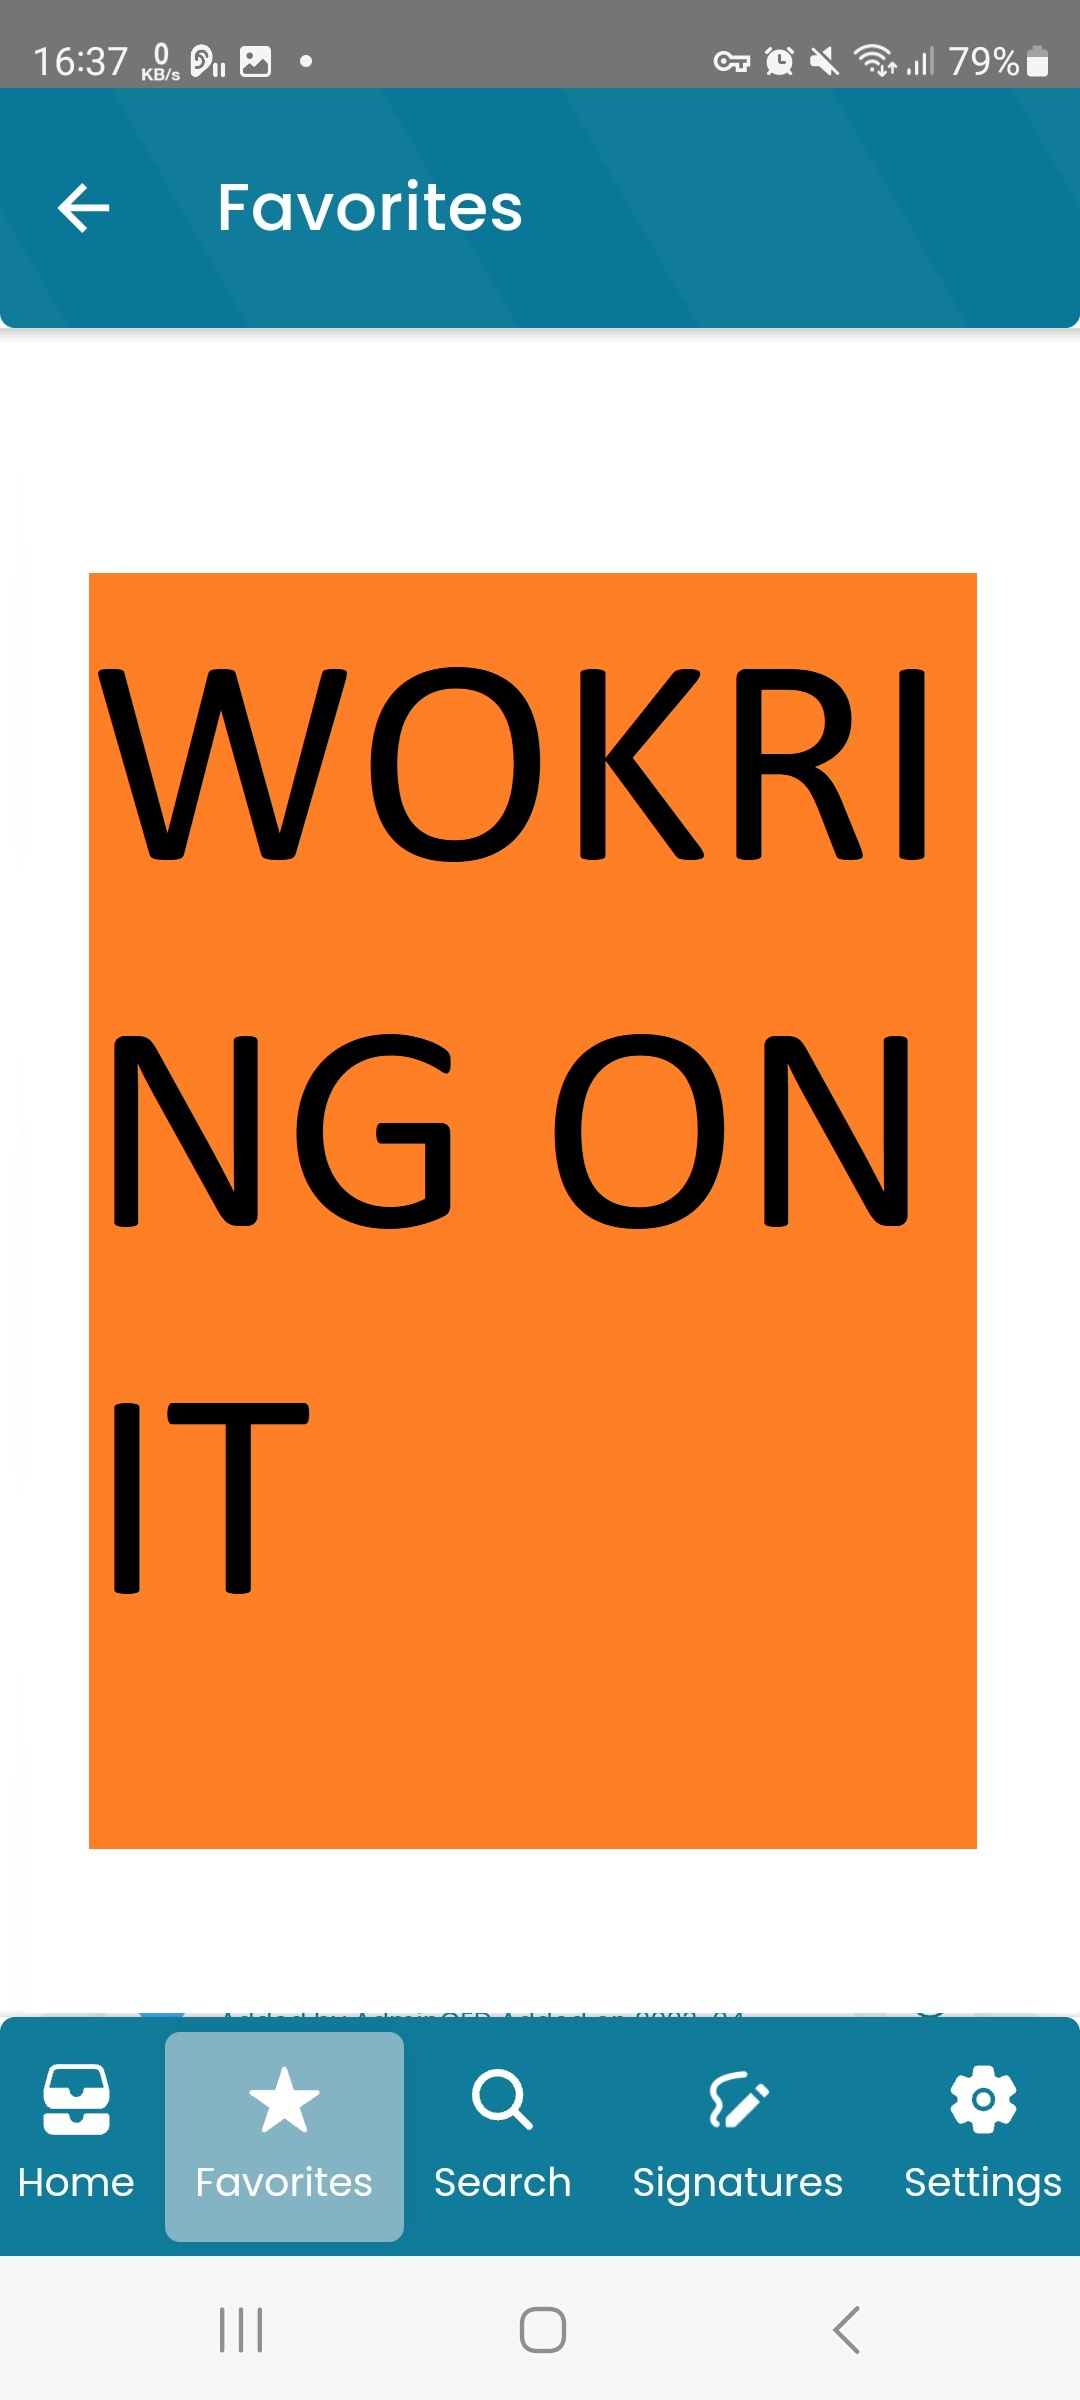
\includegraphics[width=0.35\textwidth, height=0.35\textheight,keepaspectratio=true]{add_document_files}
  \caption{Interface d'ajout de fichiers à un document}
  \label{fig:add_document_files}
\end{figure}

\textbf{• Suppression de fichiers d'un document:}

Cette capture d'écran, représente l'interface de suppression de fichiers d'un document par un utilisateur

% add image
\begin{figure}[H]
  \centering
  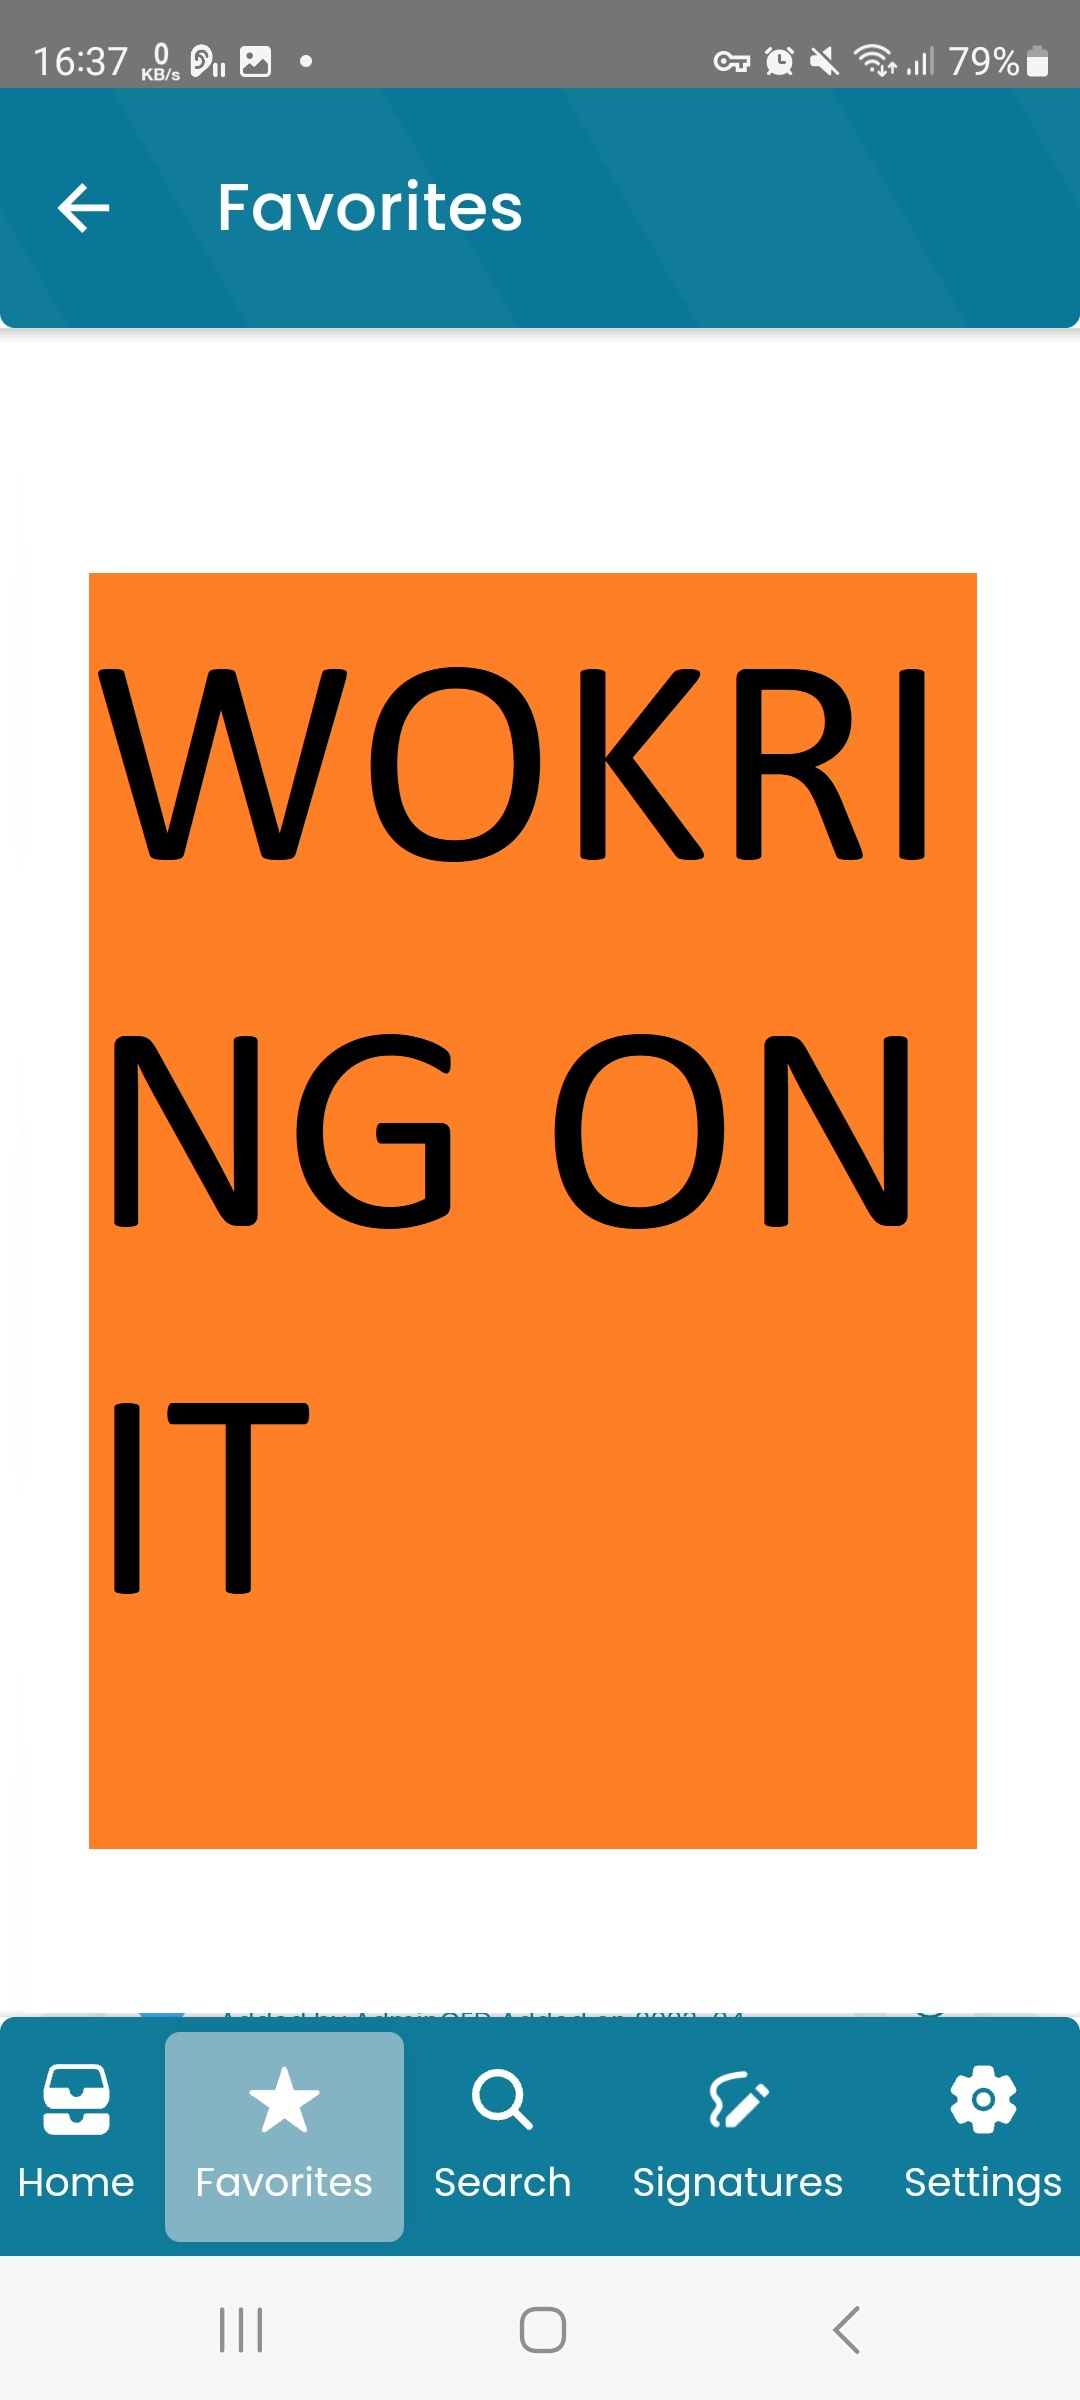
\includegraphics[width=0.35\textwidth, height=0.35\textheight,keepaspectratio=true]{delete_document_files}
  \caption{Interface de suppression de fichiers d'un document}
  \label{fig:delete_document_files}
\end{figure}


\textbf{•	Recherche d'un document:}

Cette capture d'écran, représente l'interface de recherche d'un document par un utilisateur

% add image
\begin{figure}[H]
  \centering
  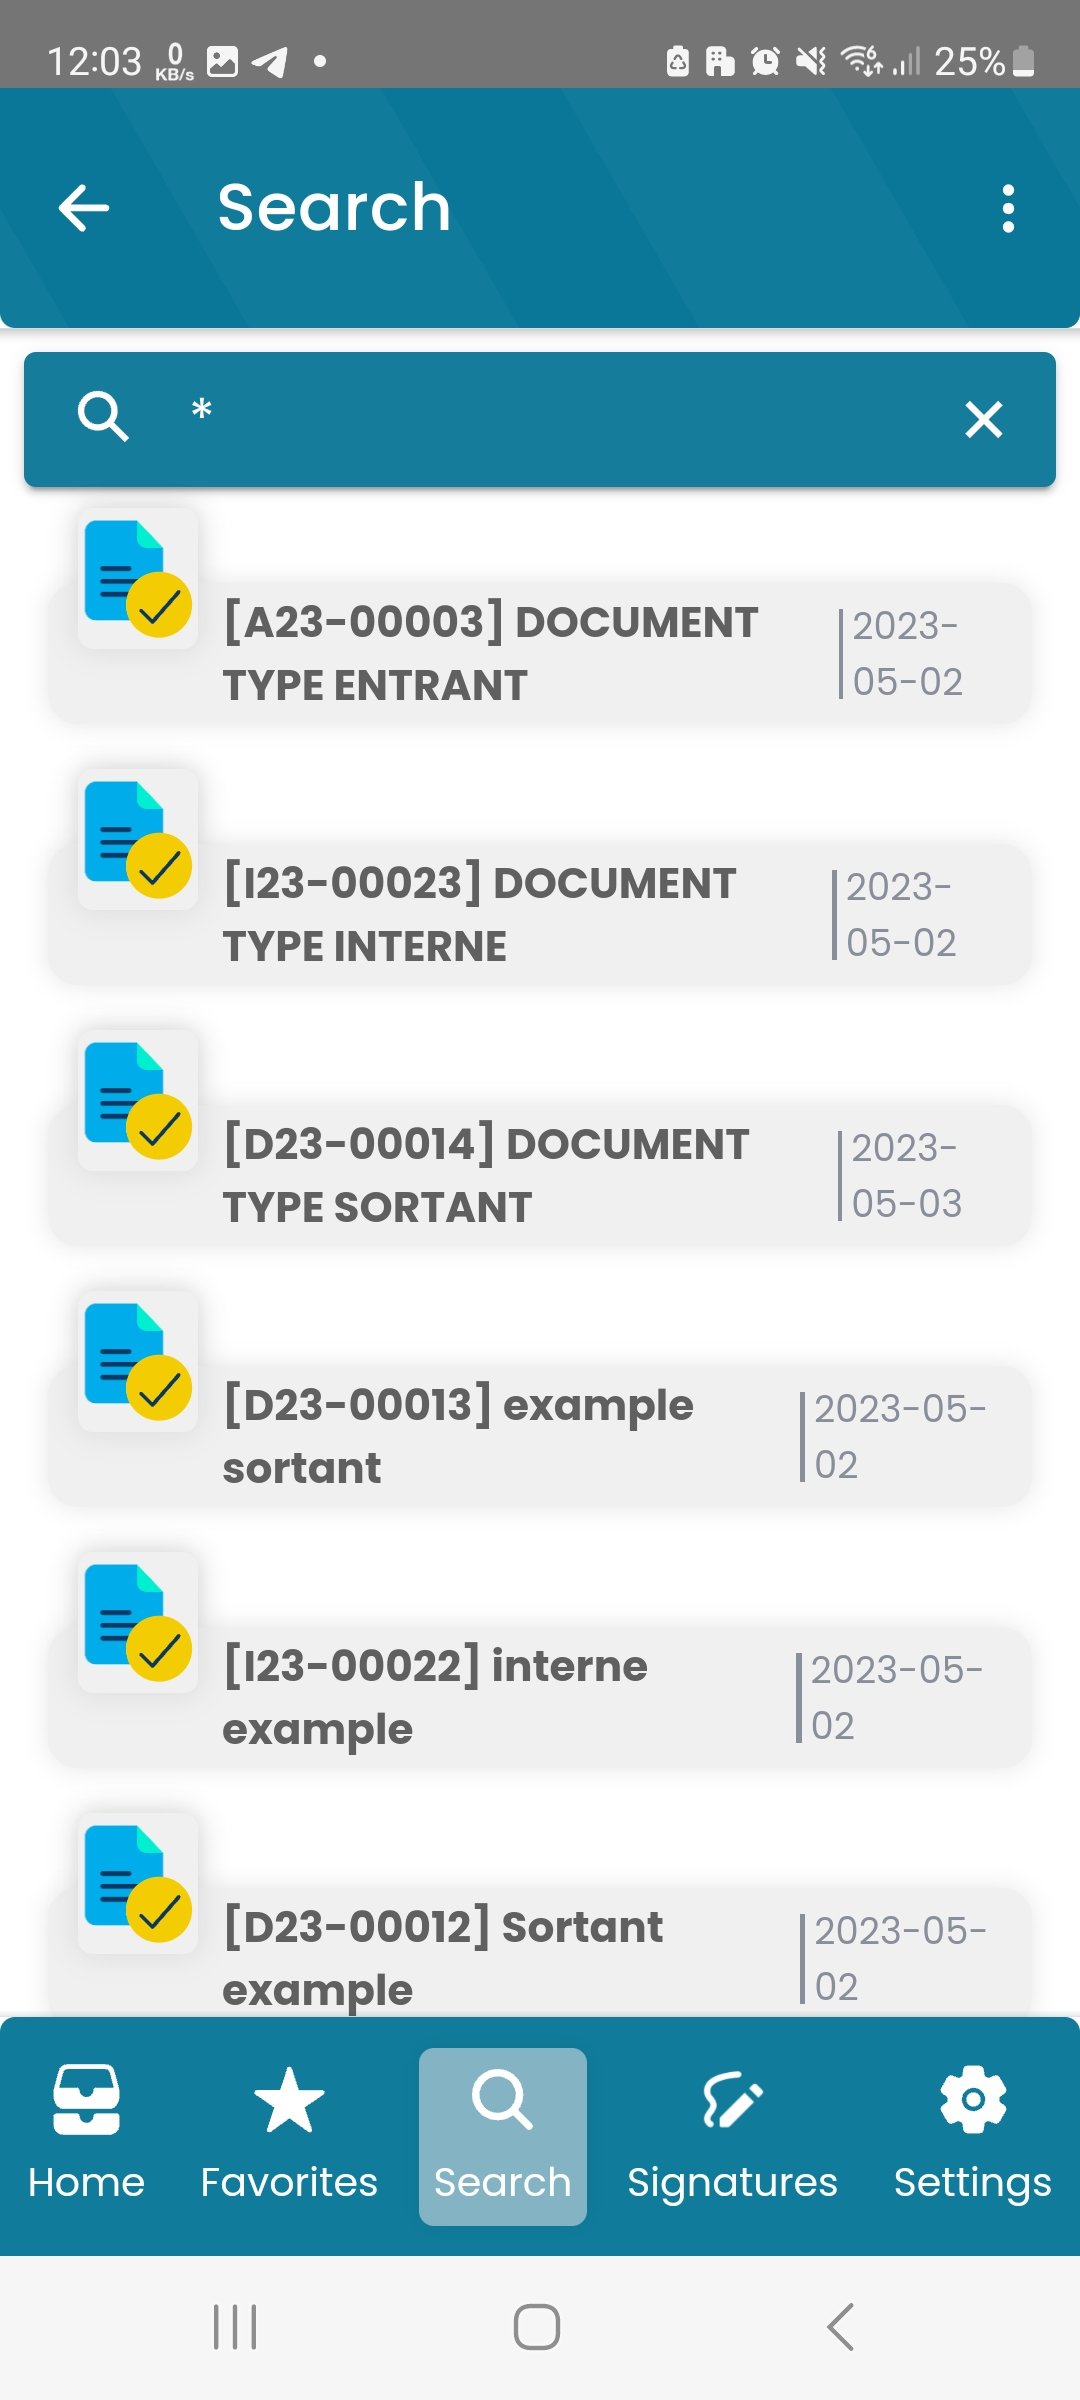
\includegraphics[width=0.35\textwidth, height=0.35\textheight,keepaspectratio=true]{search_document}
  \caption{Interface de recherche d'un document}
  \label{fig:search_document}
\end{figure}

\textbf{•	Consulter les documents en favoris:}

Cette capture d'écran, représente l'interface de consultation des documents en favoris par un utilisateur

% add image
\begin{figure}[H]
  \centering
  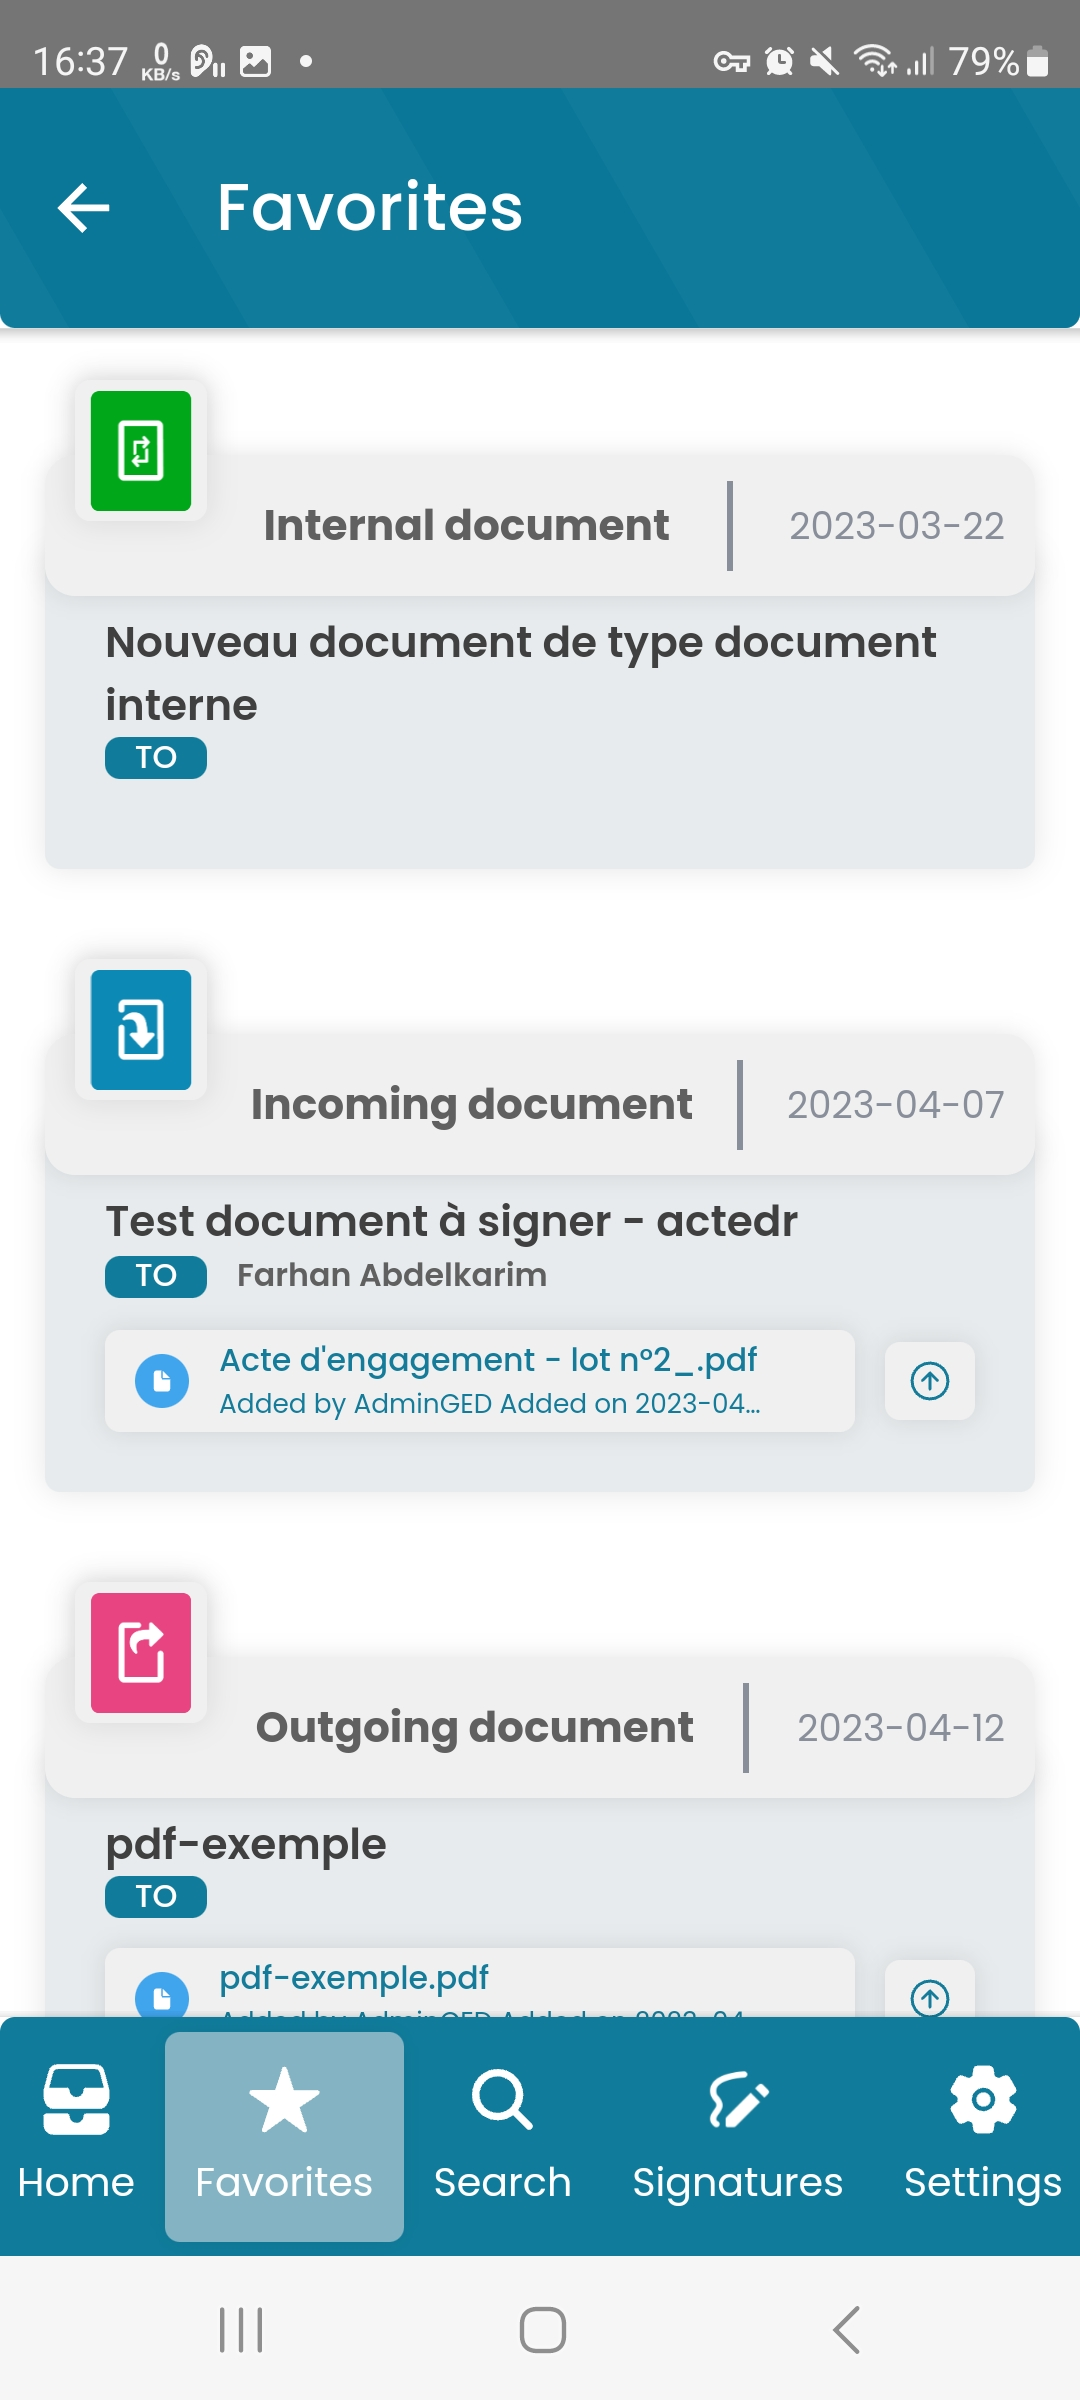
\includegraphics[width=0.35\textwidth, height=0.35\textheight,keepaspectratio=true]{consult_favoris_documents}
  \caption{Interface de consultation des documents en favoris}
  \label{fig:consult_favoris_documents}
\end{figure}

\textbf{•	Demander une tâche:}

Cette capture d'écran, représente l'interface de demande d'une tâche par un utilisateur

% add image
\begin{figure}[H]
  \centering
  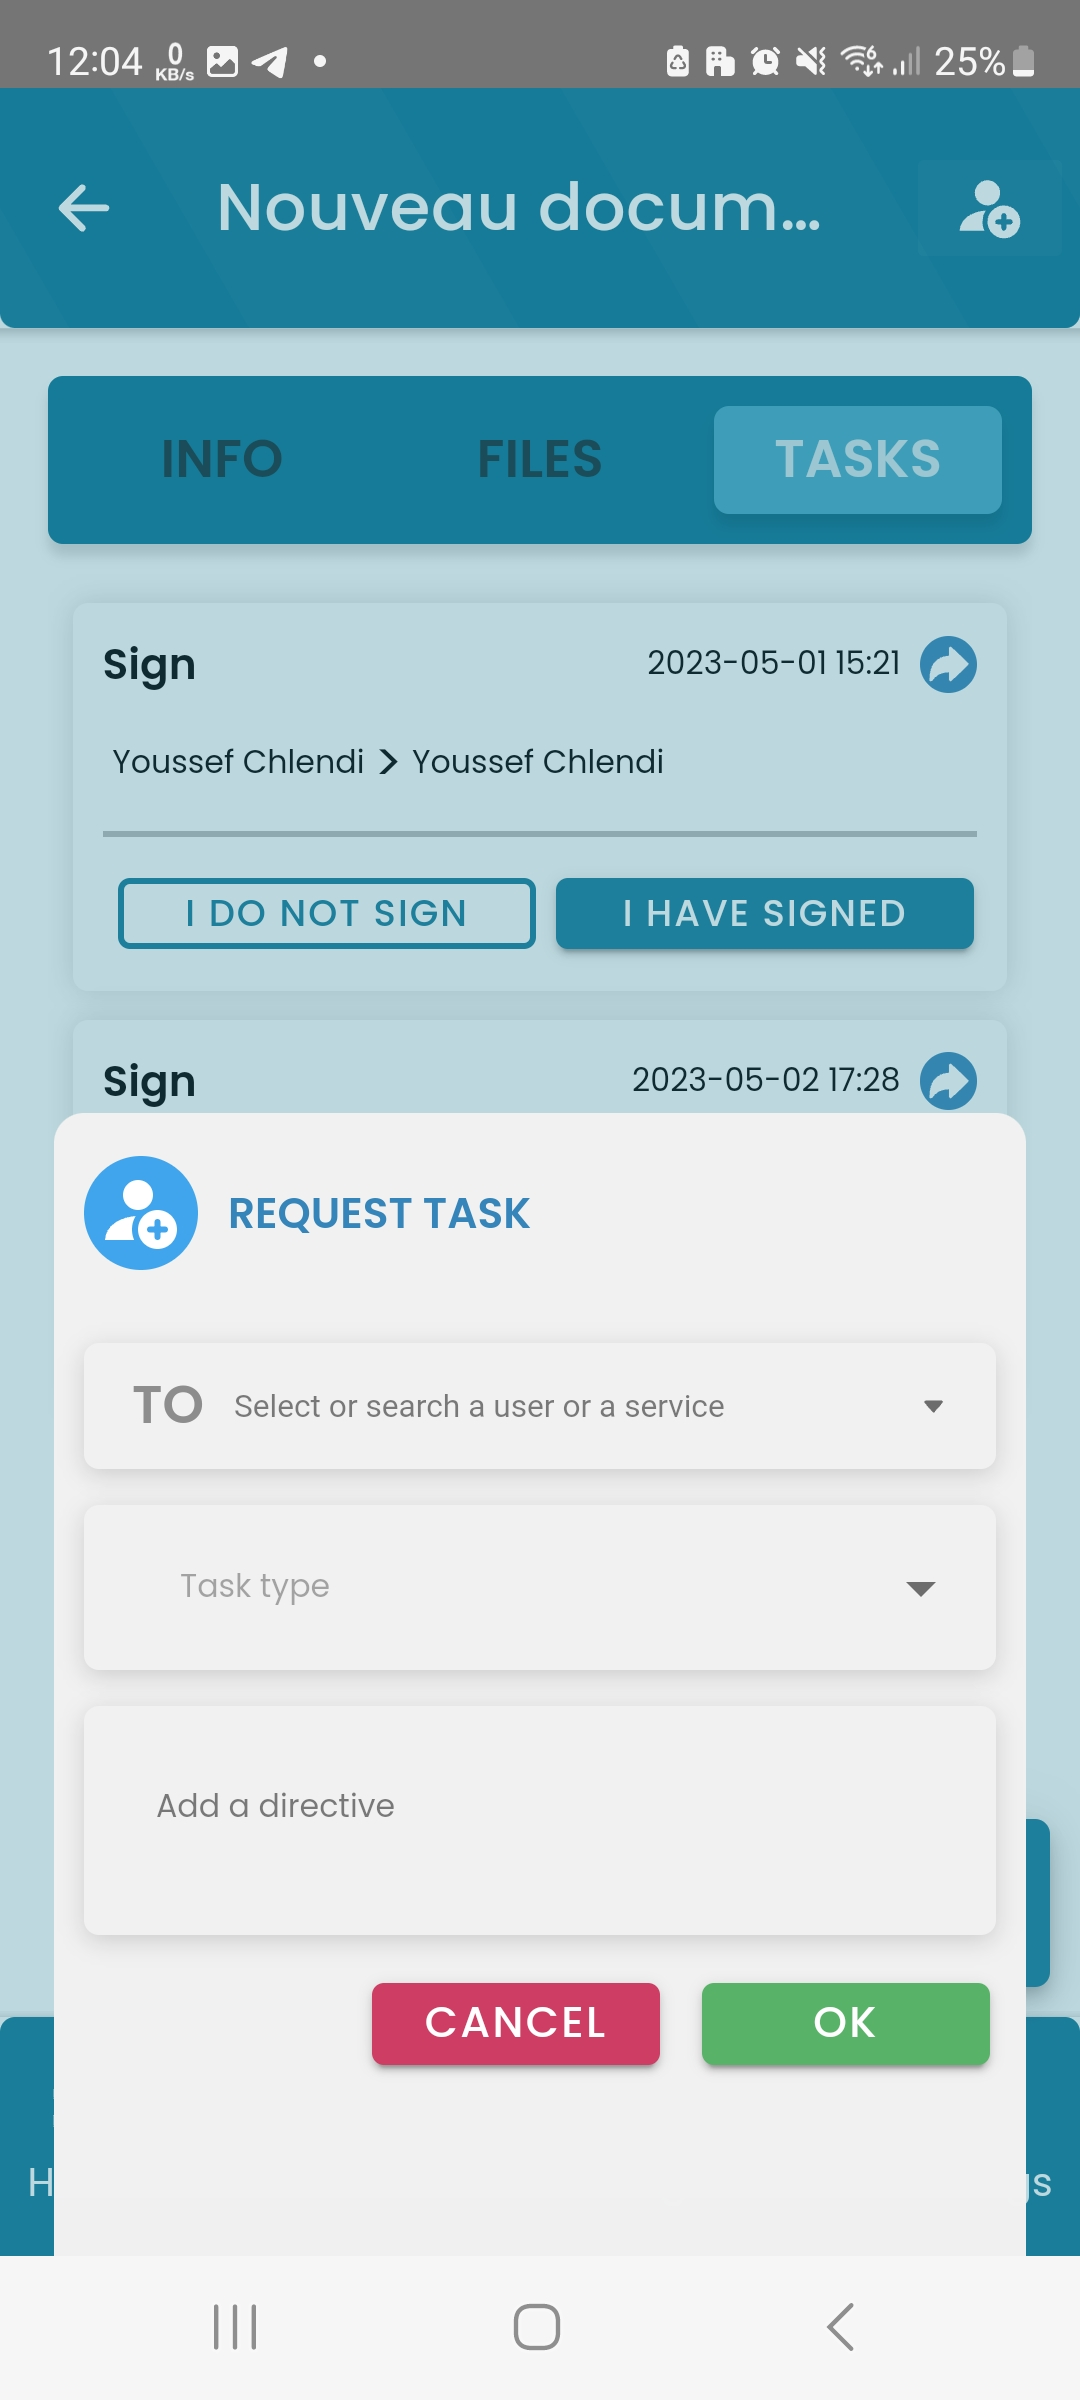
\includegraphics[width=0.35\textwidth, height=0.35\textheight,keepaspectratio=true]{ask_task}
  \caption{Interface de demande d'une tâche}
  \label{fig:ask_task}
\end{figure}

\textbf{•	Transférer une tâche:}

Cette capture d'écran, représente l'interface de transfert d'une tâche par un utilisateur

% add image
\begin{figure}[H]
  \centering
  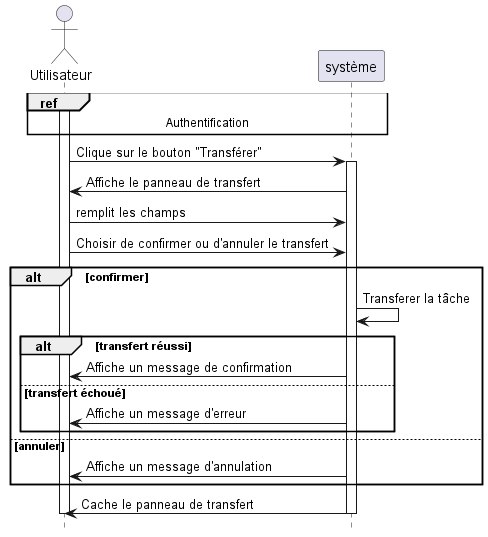
\includegraphics[width=0.35\textwidth, height=0.35\textheight,keepaspectratio=true]{transfer_task}
  \caption{Interface de transfert d'une tâche}
  \label{fig:transfer_task}
\end{figure}

\textbf{•	Terminaison d'une tâche dans un document:}

Cette capture d'écran, représente l'interface de terminaison d'une tâche dans un document par un utilisateur

% add image
\begin{figure}[H]
  \centering
  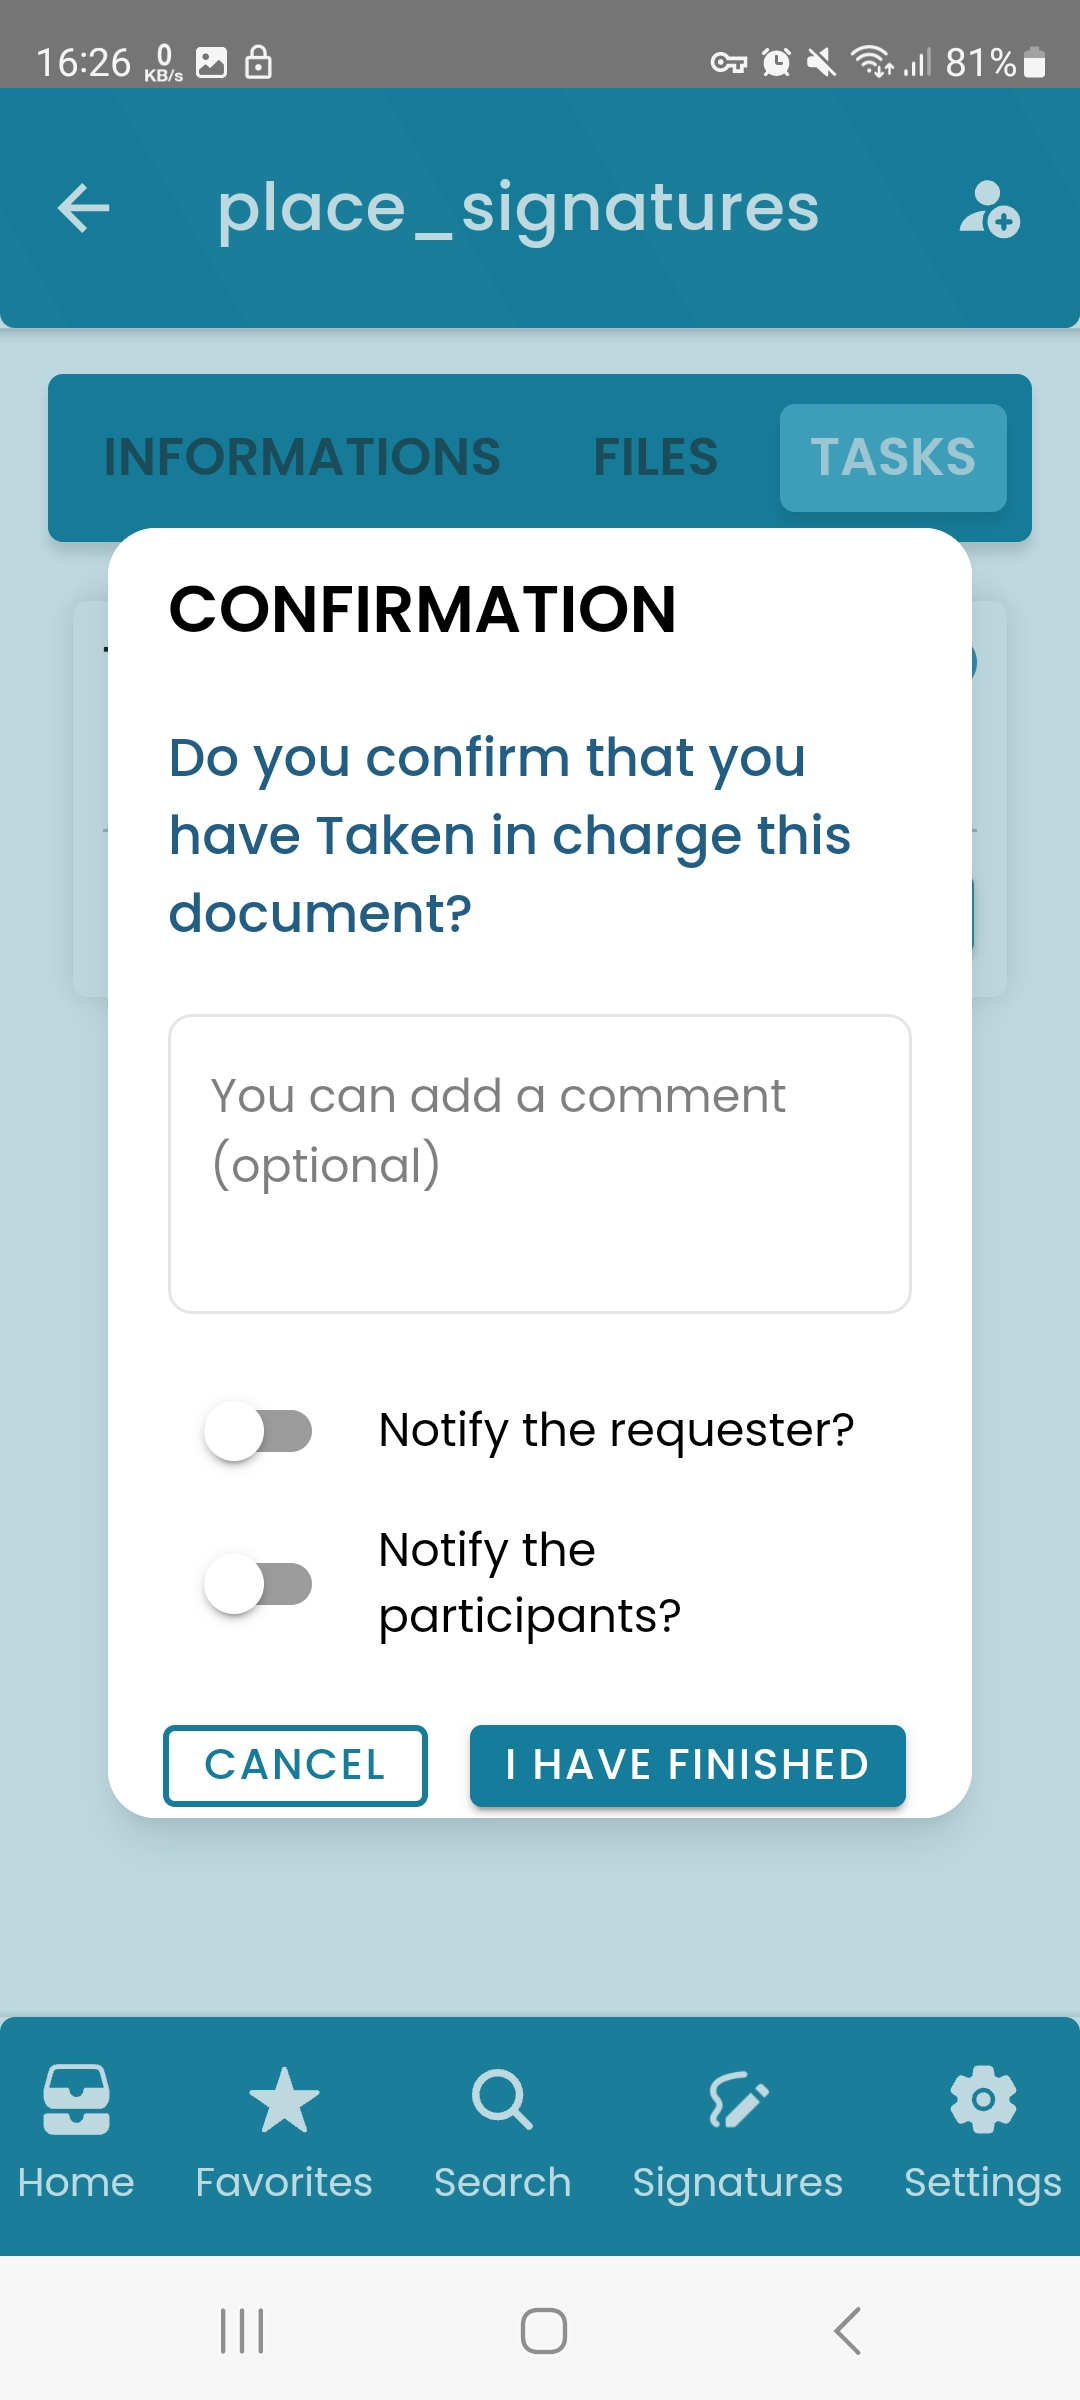
\includegraphics[width=0.35\textwidth, height=0.35\textheight,keepaspectratio=true]{end_task}
  \caption{Interface de terminaison d'une tâche dans un document}
  \label{fig:end_task}
\end{figure}




\subsection{Sprint Review:}
A la fin de ce sprint, nous avons planifié une réunion dans la société Neoledge avec le vise avis à Lille, France afin de vérifier notre démarche de travail par rapport au besoin de client tout en respectant le délai que nous avons prévu.
Nous avons fait une démonstration durant laquelle nous allons présenter notre incrément :
\begin{itemize}
  \item La consultation d'un document.
  \item La gestion des fichiers d'un document.
  \item La gestion des taches d'un document.
  \item La recherche d'un document.
  \item La consultation de la liste des documents en favoris.
\end{itemize}

\subsection{Sprint Retrospective:}

Après la Sprint Review, nous avons réfléchi à des pistes pour améliorer la qualité et l'efficacité de notre application.
\noindent\textbf{•	Ce qui a bien passé :}
Nous avons terminé le sprint dans le délai.
\noindent\textbf{•	Ce qui s'est mal passé :}
Manque de documentation de l'ionic 


% SPrint 4 visualisation et signature d'un fichier
\section{Sprint 4 (Visualisation et signature d'un fichier)}
\subsection{Sprint Goal:}
L'objectif de ce sprint est de développer et mettre en place un système de visualisation et signature d'un fichier permettant aux utilisateurs de consulter le fichier et le signer par plusieurs méthodes.


\subsection{Sprint Backlog « Visualisation et signature d'un fichier »:}

\begin{longtable}{|p{4cm}|p{7cm}|p{2cm}|p{2cm}|}
  \hline
  \textbf{Les items} &\textbf{Les tâches} & \textbf{Période} & \textbf{Sprint} \\
  \hline
  \vspace{-\baselineskip}
  \begin{enumerate}
    \setcounter{enumi}{1}
    \itemsep0em 
      \item Visualiser un fichier
      \item Signer à main un fichier
      \item Signé par glisser et déposer une image dans un fichier.
      \item Modifier la position d'une signature d'un fichier.
      \item Supprimer une signature dans fichier.
      \item Confirmer ou annuler la signature d'un fichier
  \end{enumerate}
  &
  \vspace{-\baselineskip}
  \begin{itemize}
    \itemsep0em 
    \item Préparer les interfaces sur Figma.
    \item Développer l'interface de visualisation d'un fichier.
    \item Développer un package neo-pdf-viewer qui permet d'afficher un fichier PDF à partir d'une base 64
    \item Publier le package.
    \item Intégrer le package dans notre projet.
    \item Développer une fonction qui permet de signer un main un fichier
    \item Développer le panel qui contient la liste des signatures
    \item Développer une fonction qui permet de signer par glisser et déposer une image dans un fichier.
    \item Développer une fonction qui permet de modifier la position d'une signature d'un fichier
    \item Développer une fonction qui permet de supprimer une signature d'un fichier.
    \item Développer une fonction qui permet de confirmer ou annuler la signature d'un fichier


  \end{itemize}
  &
  De 8 à 15 février  
  &
  4
  \\
  \hline
  \caption{Product Backlog Sprint 4}
  \label{tab:product_backlog_sprint_4}



\end{longtable}


\subsection{Implémentation du Sprint 4}
\textbf{•	Diagramme de cas d'utilisation du sprint 4 : « Visualisation et signature d'un fichier »}

% add image
\begin{figure}[H]
  \centering
  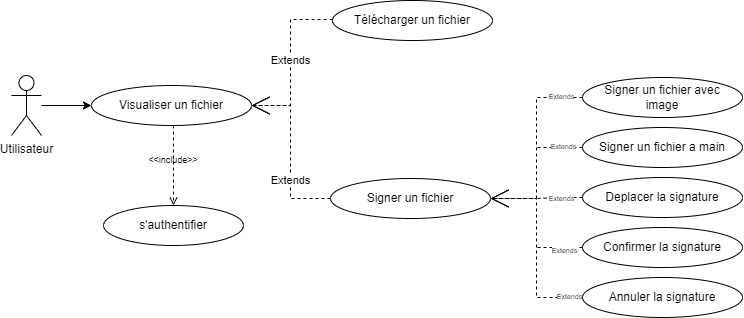
\includegraphics[width=0.8\textwidth]{use_case_documents_sprint_4}
  \caption{Diagramme de cas d'utilisation du sprint 4 : « Visualisation et signature d'un fichier »}
  \label{fig:UseCaseDiagram}
\end{figure}

\subsubsection{Analyse des besoins:}
\textbf{•	Description textuelle de cas d'utilisation « visualiser un fichier  »}

\begin{longtable}{|p{5cm}|p{10cm}|}
\hline
\textbf{Cas d'utilisation}&Visualiser un fichier\\
\hline
\textbf{Acteurs}&Utilisateur\\
\hline
\textbf{Pré Condition}&Le fichier existe\\
\hline
\textbf{Post Condition}&Le fichier est visualisé\\
\hline
\textbf{Scénario Nominal}&
\vspace{-\baselineskip}
\begin{enumerate}
    \setcounter{enumi}{1}
  \item L'utilisateur clique sur le fichier.
  \item le système affiche le fichier.
\end{enumerate}\\
\hline
\textbf{Scénario Alternatif}&
\vspace{-\baselineskip}
\begin{enumerate}
    \setcounter{enumi}{2}
    \item Aucun résultat.
\end{enumerate}\\
\hline
\textbf{Scénario d'exception}&Erreur de connexion\\
\hline
\end{longtable}

\textbf{•	Description textuelle de cas d'utilisation « Signer à main un fichier »}

\begin{longtable}{|p{5cm}|p{10cm}|}
\hline
\textbf{Cas d'utilisation}&Signer à main un fichier\\
\hline
\textbf{Acteurs}&Utilisateur\\
\hline
\textbf{Pré Condition}&Le fichier existe\\
\hline
\textbf{Post Condition}&La signature est tracée\\
\hline
\textbf{Scénario Nominal}&
\vspace{-\baselineskip}
\begin{enumerate}
    \setcounter{enumi}{1}
  \item L'utilisateur fait une longue clique sur le fichier
  \item Le système affiche un bouton pour choisir signature à main. 
  \item L'utilisateur clique sur le bouton signature à main.
  \item L'utilisateur trace sa signature.
  \item Le système affiche les 2 boutons confirmer et annuler
  \item L'utilisateur click sur le bouton confirmer
  \item Le système signe le fichier et affiche un message des succès
\end{enumerate}\\
\hline
\textbf{Scénario Alternatif}&
\vspace{-\baselineskip}
\begin{enumerate}
    \setcounter{enumi}{6}
    \item L'utilisateur click sur le bouton annuler
    \item Le tracé de la signature est effacé.
\end{enumerate}\\
\hline
\textbf{Scénario d'exception}&Erreur de connexion\\
\hline
\end{longtable}

\textbf{•	Description textuelle de cas d'utilisation « Signer par glisser et déposer une image dans un fichier »}

\begin{longtable}{|p{5cm}|p{10cm}|}
\hline
\textbf{Cas d'utilisation}&Signer par glisser et déposer une image dans un fichier\\
\hline
\textbf{Acteurs}&Utilisateur\\
\hline
\textbf{Pré Condition}&Le fichier existe\\
\hline
\textbf{Post Condition}&La signature est placée\\
\hline
\textbf{Scénario Nominal}&
\vspace{-\baselineskip}
\begin{enumerate}
    \setcounter{enumi}{1}
    \item L'utilisateur clique sur le bouton du panel.
    \item Le système affiche le panel qui contient la liste des signatures.
    \item L'utilisateur glisse une signature.
    \item L'utilisateur dépose la signature dans le fichier.
    \item Le système signe le fichier et affiche un message des succès
    
\end{enumerate}\\
\hline
\textbf{Scénario Alternatif}&
\vspace{-\baselineskip}
\begin{enumerate}
    \setcounter{enumi}{4}
    \item L'utilisateur dépose la signature hors du fichier.
\end{enumerate}\\
\hline
\textbf{Scénario d'exception}&Erreur de connexion\\
\hline
\end{longtable}


\textbf{•	Description textuelle de cas d'utilisation « Modifier la position d'une signature d'un fichier »}

\begin{longtable}{|p{5cm}|p{10cm}|}
\hline
\textbf{Cas d'utilisation}&Modifier la position d'une signature d'un fichier\\
\hline
\textbf{Acteurs}&Utilisateur\\
\hline
\textbf{Pré Condition}&La signature est placée et l'utilisateur n'a pas encore confirmer les changements\\
\hline
\textbf{Post Condition}&La position de la signature est modifiée\\
\hline
\textbf{Scénario Nominal}&
\vspace{-\baselineskip}
\begin{enumerate}
    \setcounter{enumi}{1}
    \item L'utilisateur clique sur la signature et la déplace.
    \item Le système modifie la position de la signature.
\end{enumerate}\\
\hline
\textbf{Scénario Alternatif}&
\vspace{-\baselineskip}
\begin{enumerate}
    \setcounter{enumi}{4}
    \item L'utilisateur dépose la signature hors du fichier.
    \item Le système annule les changements.
\end{enumerate}\\
\hline
\textbf{Scénario d'exception}&Erreur de connexion\\
\hline
\end{longtable}

\textbf{•	Description textuelle de cas d'utilisation « Supprimer une signature d'un fichier  »}

\begin{longtable}{|p{5cm}|p{10cm}|}
\hline
\textbf{Cas d'utilisation}&Supprimer une signature d'un fichier \\
\hline
\textbf{Acteurs}&Utilisateur\\
\hline
\textbf{Pré Condition}&La signature est placée et l'utilisateur n'a pas encore confirmer les changements\\
\hline
\textbf{Post Condition}&La signature est supprimée\\
\hline
\textbf{Scénario Nominal}&
\vspace{-\baselineskip}
\begin{enumerate}
    \setcounter{enumi}{1}
    \item L'utilisateur déplace la signature dans la zone de suppression.
    \item Le système supprime la signature d'un fichier
\end{enumerate}\\
\hline
\textbf{Scénario Alternatif}&
\vspace{-\baselineskip}
\begin{enumerate}
    \setcounter{enumi}{4}
    \item L'utilisateur dépose la signature hors du fichier.
    \item Le système annule les changements.
\end{enumerate}\\
\hline
\textbf{Scénario d'exception}&Erreur de connexion\\
\hline
\end{longtable}


\textbf{•	Description textuelle de cas d'utilisation « Confirmer ou annuler les changements d'un fichier »}

\begin{longtable}{|p{5cm}|p{10cm}|}
\hline
\textbf{Cas d'utilisation}&Confirmer ou annuler les changements d'un fichier\\
\hline
\textbf{Acteurs}&Utilisateur\\
\hline
\textbf{Pré Condition}&Le fichier est modifié\\
\hline
\textbf{Post Condition}&Les changements sont enregistrés ou annulés\\
\hline
\textbf{Scénario Nominal}&
\vspace{-\baselineskip}
\begin{enumerate}
    \setcounter{enumi}{1}
    \item L'utilisateur clique sur le bouton confirmer.
    \item Le système enregistre les changements et affiche un message des succès.
\end{enumerate}\\
\hline
\textbf{Scénario Alternatif}&
\vspace{-\baselineskip}
\begin{enumerate}
    \setcounter{enumi}{1}
    \item L'utilisateur clique sur le bouton annuler.
    \item Le système annule les changements.
\end{enumerate}\\
\hline
\textbf{Scénario d'exception}&Erreur de connexion\\
\hline
\end{longtable}

% \textbf{•	Description textuelle de cas d'utilisation « Afficher la liste des signatures »}

% \begin{longtable}{|p{5cm}|p{10cm}|}
% \hline
% \textbf{Cas d'utilisation}&Afficher la liste des signatures\\
% \hline
% \textbf{Acteurs}&Utilisateur\\
% \hline
% \textbf{Pré Condition}&Le fichier existe\\
% \hline
% \textbf{Post Condition}&La liste des signatures est affichée\\
% \hline
% \textbf{Scénario Nominal}&
% \vspace{-\baselineskip}
% \begin{enumerate}
%     \setcounter{enumi}{1}
%     \item L'utilisateur glisse la liste des signatures.
%     \item Le système affiche le panel qui contient la liste des signatures.
% \end{enumerate}\\
% \hline
% \textbf{Scénario d'excepetion}&Erreur de connexion\\
% \hline
% \end{longtable}


\subsubsection{Analyse détaillée}

DIAGRAMAT HNI 

\subsubsection{Conception}

Après la présentation des diagrammes d'analyse, nous avons présenté dans cette partie les diagrammes de conception.
Nous allons présenter dans cette partie les diagrammes de conception de sprint 4.

\textbf{•	Diagramme de classe de conception de sprint 4 : « Visualisation et signature
d'un fichier »}

% add image
\begin{figure}[H]
  \centering
  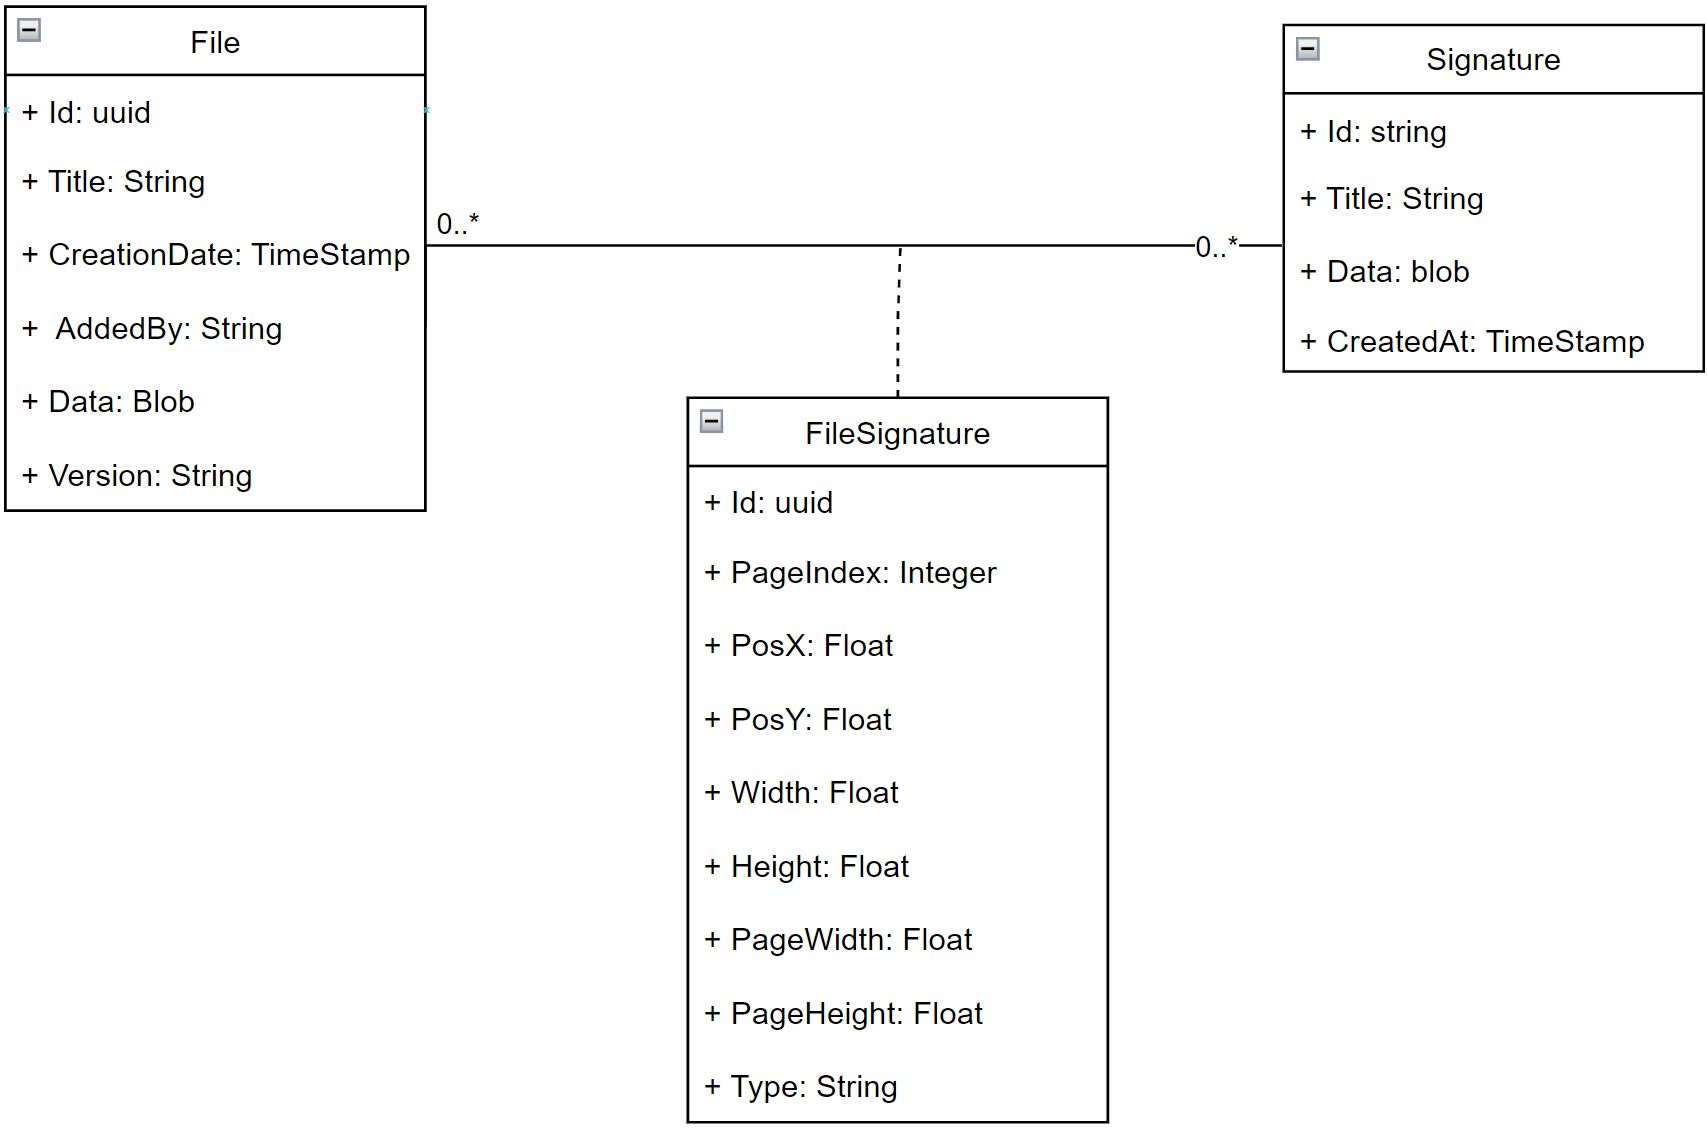
\includegraphics[width=0.8\textwidth, height=0.8\textheight, keepaspectratio=true]{class_diagram_sprint4}
  \caption{Diagramme de classe de conception de sprint 2 : « Visualisation et signature
  d'un fichier »}
  \label{fig:ClassDiagramSprint4}
\end{figure}

\subsubsection{Réalisation}

\subsection{Sprint review:}


A la fin de ce sprint, nous avons planifié une autre réunion dans la société Neoledge  afin de vérifier notre démarche de travail par rapport au besoin de client tout en respectant le délai que nous avons prévu.

Nous avons fait une démonstration durant laquelle nous allons présenter notre incrément :
\begin{itemize}
  \item La visualisation d'un fichier.
  \item La signature à main d'un fichier.
  \item La signature par glisser et déposer une image dans un fichier.
  \item La modification de la position d'une signature d'un fichier.
  \item La suppression d'une signature d'un fichier.
  \item La confirmation ou l'annulation de la signature d'un fichier
\end{itemize}

\subsection{Sprint retrospective:}

Après la Sprint Review, nous avons réfléchi à des pistes pour améliorer la qualité et l'efficacité de notre application.


\noindent\textbf{•	Ce qui s'est bien passé :}
Nous avons terminé le sprint dans le délai.
\noindent\textbf{•	Ce qui s'est mal passé :}
\begin{itemize}
  \item Manque de documentation de l'ionic
  \item Difficulté tu développement du package neo-pdf-viewer et son intégration dans notre projet
  \item Difficultés de déposer la signature à la position exacte.
\end{itemize}

